\documentclass[oneside]{mgr}
%opcje klasy dokumentu mgr.cls zostały opisane w dołączonej instrukcji

%poniżej deklaracje użycia pakietów, usunąć to co jest niepotrzebne
%\usepackage{polski}       %przydatne podczas składania dokumentów w
%j. polskim 
\usepackage[polish]{babel} %alternatywnie do pakietu
%polski, wybrać jeden z nich
\usepackage[utf8]{inputenc} %kodowanie znakĂłw, zaleĹźne od systemu
\usepackage[T1]{fontenc} %poprawne składanie polskich czcionek
%\usepackage{polski}
%pakiety do grafiki
\usepackage{graphicx}
\usepackage{subfigure}
\usepackage{psfrag}
\let\lll\undefined
%pakiety dodające dużo dodatkowych poleceń matematycznych
\usepackage{amssymb}
\usepackage{amsmath}

\usepackage{amsfonts}

%pakiety wspomagające i poprawiające składanie tabel
\usepackage{supertabular}
\usepackage{array}
\usepackage{tabularx}
\usepackage{hhline}
\usepackage{multirow}
\usepackage{changepage}

\usepackage{tabto}
\usepackage{listings} 
%pakiet wypisujący na marginesie etykiety równań i rysunków
%zdefiniowanych przez \label{}, chcąc wygenerować finalną wersję
%dokumentu wystarczy usunąć poniższą linię
\usepackage{showlabels}

%definicje własnych poleceń
\newcommand{\R}{I\!\!R} %symbol liczb rzeczywistych, działa tylko w
                        %trybie matematycznym
\newtheorem{theorem}{Twierdzenie}[section] %nowe otoczenie do
                                           %składania twierdzeń

%dane do złożenia strony tytułowej
\title{Badanie wydajności algorytmów z kluczem symetrycznym w bibliotece kryptograficznej WolfSSL na platformie STM32F2}
\engtitle{Performance analysis of symmetric-key algorithms in WolfSSL cryptographic library on STM32F2 platform}
\author{Michał Stroka}
\supervisor{dr inż. Grzegorz Budzyń, I-6}

\date{2017} %standardowo u dołu strony tytułowej umieszczany jest
%bieżący rok, to polecenie pozwala wstawić dowolny rok

%poniżej jest lista kierunków i specjalności na wydziale elektroniki,
%naleĚźy wybrać właściwe lub dopisać jeśli nie ma odpowiednich
\field{Automatyka i Robotyka (AIR)}

\specialisation{Komputerowe sieci sterowania (ARK)}
%\graphicspath{ {./img/} }
\sloppy
%tutaj zaczyna się właśniwa treść	 dokumentu
\begin{document}
\bibliographystyle{plabbrv} %tylko gdy uĚźywamy BibTeXa, ustawia polski
                            %styl bibliografii

\maketitle

\tableofcontents %spis treści

%poniżej znajduje się przykładowa treść dalszej części dokumentu,
%zainteresowanych zachęcam do rozszyfrowania frazy "Lorem ipsum" :)
\chapter{Wstęp}
Już w czasach starożytnych ludzie zaczeli dostrzegać potrzebę komunikacji między dwiema osobami bez możliwości przechwycenia i odczytania jej przez osoby trzecie. Najstarszym znanym szyfrem jest szyfr Cezara, którym Juliusz Gajusz Cezar w pierwszym wieku p.n.e. szyfrował korespondencję. Był to tak zwany szyfr przesuwający z przesunięciem 3. Każda litera ,,a'' była zamieniana na ,,d'', ,,b'' na ,,e'' itd. Oczywiście taki szyfr był bardzo łatwy do złamania, jednak w czasach gdy umiejętność czytania była rzadkością, zwłaszcza wśród przeciwników Rzymu, zupełnie wystarczał. Później przez całą historię trwał ciągły rozwój kryptologii - nauki o przekazywaniu informacji w sposób zabezpieczony przed niepowołanym dostęp. Ponieważ ludzie zdawali sobie sprawę że np. w czasie wojny zdobycie informacji o ruchach przeciwnika może przesądzić o losie bitwy, to szeregi matematyków wynajdowały nowe metody szyfrowania i jednocześnie usiłowały złamać te już istniejące. Prawdopodobnie najbardziej znaną maszyną szyfrującą była Enigma - niemiecka maszyna szyfrująca, która zostałą złamana przez 3 polskich matematyków: Mariana Rejewskiego, Henryk Zygalski i Jerzego Różyckiego. Równolegle do zatajania treści wiadomości rozwijały się techniki ukrywania samego faktu wysyłania wiadomości. Na początku XX. wieku Niemcy dysponowali techniką, która pozwalała na sfotografowanie kartki rozmiaru A4 i pomniejszenie zdjęcia do rozmiaru pojedynczej kropki w tekście, a następnie mogła być za pomocą mikroskopu z powrotem powiększona. Tak przekazana książka z kilkoma tajnymi kropkami nie budziła podejrzeń nawet gdy zostałą przechwycona przez przeciwników.\\
W dzisiejszym świecie, gdy wraz z rozwojem i rozpowszechnieniem się komputerów tysiące informacji są przekazywane tajność korespondencji wydaje się być kluczowa. Obecnie problem dotyczy nie tylko najbardziej wpływowych osób na świecie i wymiany informacji pomiędzy nimi, ale każdego z nas. Niezależnie czy logujemy się do banku, wysyłamy maile/SMSy, przesyłamy pliki po sieci czy wpisujemy gdzieś nasze dane osobowe każdy z nas ma nadzieję, że te wrażliwe dane będą dostępne tylko dla adresata końcowego i nie zostaną zrozumiane przez osoby postronne. Dodatkowo wraz z rozwojem elektroniki coraz częściej mamy doczynienia z komunikacją między dwoma urządzeniami np. komunikacja między kartą płatniczą, a terminalem, czy wymiana informacji między podzespołami w autonomicznych pojazdach. Tutaj również ważne jest, aby komunikacja była tajna i nie była podmieniona, gdyż może spowodować to zmianę kwoty i/lub rachunku obciążanego w przypadku kart, i katastrofę w ruchu drogowym/lotniczym w przypadku pojazdów. Obecnie istnieje wiele standardowych szyfrów kryptograficznych, które według obecnej wiedzy są nie do złamania w rozsądnym czasie. Wydajność niektórych z nich zostanie zbadana w tej pracy.

\chapter{Cel pracy}

Celem pracy magisterskiej jest zbadanie wydajności algorytmów symetrycznych w bibliotece kryptograficznej WolfSSL na platformie STM32F2. Praca zakłada kompilację biblioteki na wybraną platformę, zaprojektowanie i stworzenie środowiska testowego pozwalającego na  przeprowadzenie pomiarów w sposób łatwy i automatyczny, porównanie czasów wykonywania algorytmów tylko w procesorze oraz z użyciem wbudowanych procesorów kryptograficznych, a także stworzenie własnej implementacji niektórych algorytmów i porównania ich prędkości.
\chapter{Konfiguracja środowiska}

Platformą testową, na której badana jest wydajność biblioteki WolfSSL to płytka testowa STM3221G-EVAL z mikroprocesorem STM32F217IG. Procesor ten posiada specjalnie dedykowane hardware'owe jednostki kryptograficzne, które pozwalają na znaczne przyspieszenie niektórych algorytmów dzięki sprzętowemu wykonywaniu części obliczeń.  Algorytmy symetryczne, dla których wsparcie sprzętowe posiada wyżej wymieniony procesor, to AES, DES, MD5 i SHA-1. Wszystkie one mogą być wykorzystywane przez bibliotekę WolfSSL. W pracy zostaną porównane wydajności algorytmów z i bez użycia kryptojednostek oraz porównanie czasów z własną implementacją algorytmów.
\begin{center}
\begin{figure}[h]
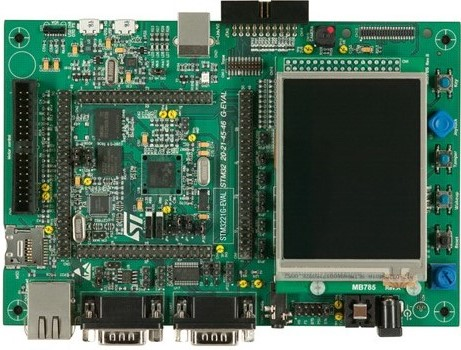
\includegraphics[width = \textwidth]{stm3221g-eval}
\caption{Płytka testowa stm3221g-eval}
\end{figure}

\end{center}



\section{Struktura katalogów w projekcie}

Struktura katalogów w projekcie jest następująca 
\begin{itemize}
\item{ldscript}
\item{libs}
\begin{itemize}
\item{Drivers}
\begin{itemize}
\item{CMSIS}
\item{STM32F2\_HAL\_Driver}
\end{itemize}
\item{wolfssl-3.9.10}
\end{itemize}
\item{misc}
\item{test\_vectors}
\item{workspace}
\begin{itemize}
\item{src}
\item{inc}
\item{build}
\end{itemize}
\end{itemize}

W folderze ldscripts znajdują się skrypty linkera. To one definiują m.in. ile pamięci RAM/flash jest dostępne w procesorze oraz definiują podział pamięci na stertę i stos.\\
W folderze libs, podkatalogu Drivers znajdują się dwie bilioteki procesora STM32F2. Stanowią one swoisty interfejs do części hardwerowej procesora. Pozwalają na zarządzanie np. tatktowania zegarem procesora, konfiguracją timerów, obsługą krpytoprocesorów (badany procesor ma specjalnie dedykowane kryptojednostki wykonujące niektóre algorytmy np. AES, SHA-1) czy portów GPIO.\\
W folderze libs, podkatalogu wolfssl-3.9.10 znajdują się pliki źródłowe badanej biblioteki wolfSSL oraz zbudowana biblioteka.\\
W folderze misc znajdują się różne pliki, które nie mają swoich predefiniowanych katalogów. Są tam pliki opisujące sposób biblioteki wolfSSL, czy konfiguracji połączenia między komputerem klasy PC, a płytką testową z mikrokontrolerem STM32.\\
Folder test\_vectors zawiera dane testowe, które służą do badania wydajnośći poszczególnych implementacji algorytmów. Dzięki wspólnym danym wejściowym, wyniki mogą być bezpośrednio porównywane.\\
W Folderze workspace, w poczególnych podkatalogach znajdują się pliki źródłowe z moją własną implementacją poszczególnych algorytmów, pliki nagłówkowe, a w katalogu pliki powstające w momencie budowania całego projektu (pliki obiektowe oraz plik ELF, który jest wgrywany do procesora).
\section{Instalowanie IDE do programowania STM32}

W pracy zdecydowano się użyć toolchain'u dedykowanego do STM32 dla aplikacji bare metalowych (bez nadrzędnego systemu operacyjnego) GNU ARM Embedded Toolchain. Posiada on kompilator arm-gcc-none-eabi, który wspiera kompilację na większość platform z rodzin Cortex-M i Cortex-R, w szczególności na interesujący nas Cortex-M7. Posiada też wbudowany debugger GDB (GNU Debugger), który pozwala podejrzeć co dzieje się wewnątrz programu (aktualne wartości zmiennych, rejestrów procesora, adresów w pamięci, licznik programu) oraz pozwala na sterowanie jego przebiegiem przez zatrzymywanie cyklu programu w kluczowych momentach przez brakepointy, czy przechodzenie ,,krok po kroku'' między instrukjami.\\
Do zarządzania procesem budowania został użyty program make. Pozwala on na łatwe ustawianie reguł w jaki sposób należy budować poszczególne pliki, ustawia ścieżki do dołączania plików, czy wybór wersji biblioteki z której chcemy korzystać. Dzięki dobremu plikowi Makefile można posiadać wiele konfiguracji do budowania programu i wybierać odpowiednią za pomocą opcji wywołania programu make np. \textit{make all LIBRARY=wolfssl\_no\_hardwarecrypto }

Do wgrywania zbudowanego program został użyty programator SEGGER, który jest już wbudowany w płytkę testową.

Ostantim używanym programem jest OpenOCD (Open On Chip Debugger). Za pomocą interfejsu JTAG dostępnego na płytce komunikuje się on z procesorem, umożliwia semihosting czyli przekazywanie danych z/do komputera w czasie pracy mikroprocesora.

\section{Kompilowanie biblioteki}

Pierwszym krokiem do zbudowania biblioteki jest wybór platformy, na której kod będzie wykonywany. W tym celu edytujemy plik \textit{settings.h} znajdujące się w katalogu \textit{wolfssl-3.9.10/wolfssl/wolfcrypt/}. Ponieważ naszą platformą jest STM32F2, to w pliku odkomentowujemy \#define WOLFSSL\_STM32F2 (linia 92). W późniejszej fazie pracy z biblioteką, okazało się że w pliku trzeba też usunąć \#define KEIL\_INTRINSICS (linia 766). WolfSSL w wersji 3.9.10 jawnie zakłada, że jedynym kompilatorem służącym do zbudowania biblioteki jest płatny kompilator Keil'a. Po usunięciu tej instrukcji dodającej funkcje kompilatora Keil, biblioteka kompiluje się również przy użyciu arm-gcc-none-eabi oraz dowolnych innych kompilatorów języka C na platformę STM32F2.
W celu dalszej konfiguracji biblioteki powstał następujący skrypt bashowy:\\
\texttt{
CC=/c/GNU\_Tools\_ARM\_Embedded/4.9\_2015q3/bin/arm-none-eabi-gcc\\
AR=/c/GNU\_Tools\_ARM\_Embedded/4.9\_2015q3/bin/arm-none-eabi-ar\\
RANLIB=/c/GNU\_Tools\_ARM\_Embedded/4.9\_2015q3/arm-none-eabi/bin/ranlib\\
LDFLAGS=" -lc -specs=nosys.specs"\\
CFLAGS="-mcpu=cortex-m3 -march=armv7-m -mthumb -mlittle-endian -DNO\_WRITEV \\-DWOLFSSL\_USER\_IO -DWOLFCRYPT\_ONLY\\-I/Drivers/CMSIS/Include\\-I/Drivers/CMSIS/Device/ST/STM32F2xx/Include\\-I/Drivers/STM32F2xx\_StdPeriph\_Lib\_V1.1.0/Libraries/STM32F2xx\_StdPeriph\_Driver/src\\-I/Drivers/STM32F2xx\_HAL\_Driver/Inc \\-I/Drivers/STM32F2xx\_HAL\_Driver/Src\\-I/Drivers/STM32F2xx\_StdPeriph\_Lib\_V1.1.0/Libraries/STM32F2xx\_StdPeriph\_Driver/inc"\\
./configure --host=arm-none-eabi CC=\$CC AR=\$AR RANLIB=\$RANLIB LDFLAGS="\$LDFLAGS" CFLAGS="\$CFLAGS"	
}
\\Zmienna CC przechowuje ścieżkę do kompilatora arm-none-eabi-gcc
\\Zmienna AR przechowuje ścieżkę do programu ar, służącego do tworzenia/modyfikowania/wyciągania danych z archiwum
\\Zmienna RANLIB przechowuje ścieżkę do programu ranlib, który tworzy indeksowaną listę symboli w archiwum
\\Zmienna LDFLAGS zawiera dodatkowe flagi dla linkera. Flaga -lc dodaje bibliotekę libc.a do kompilacji, flaga -specs=nosys.specs oznacza, że aplikacja będzie działała na platformie bez systemu operacyjnego i funkcje systemowe jak np. malloc muszą być dodane przez kompilator
\\Zmienna CFLAGS zawiera dodatkowe zmienne dla kompilatora. Zmienna -mcpu=cortex-m3 oznacza że program będzie wykonywany na platformie Cortex-M3, -march=armv7-m określa architekturę procesora jako ARMv7-M, -mthumb dodaje rozszerzony zestaw instrukcji asemblerowych Thumb, -mlittle-endian oznacza że zmienne w procesorze są pzechowywane w formacie little endian (najmniej znaczący bit jest najmłodszy). Flagi -NO\_WRITEV -WOLFSSL\_USER\_IO oznaczają, że w systemie nie ma żadnych instrukcji wejścia/wyjścia, a użytkownik posiada swoje funkcje IO (eng. input/output). Kolejne flagi zaczynające się od I/ zawierają ścieżki do plików nagłóWkowych i żródłowych bibliotek STM32F2.
\\Ostatnia linia skryptu wywołuje inny skrypt dostarczany przez WolfSSL, który przetwarza wszystkie dane i tworzy własny plik Makefile.
Tak przygotowana biblioteka jest już prawie gotowa do kompilacji. Ostatnim krokiem jest poprawienie stworzonego pliku Makefile. Z flag kompilacji należy usunąć -fpie. Jest to flaga Position Independent Executable, która normalnie powoduje że kod biblioteki może być wpisany w dowolne miejsce w pamięci. Niestety w przyapdku platformy STM32F2 powodowało to, że w czasie wykonywania programu procesor próbował odczytywać nieistniejące rejestry pamięci, co koóńczyło się zawieszeniem procesora, przez uruchomienie procedury HardFault\_handler. Znalezione rozwiązanie zostało przedstawione supportowi WolfSSL i została wydana nowa wersja biblioteki 3.10.0, która domyślnie nie wstawia tej flagi. Po dokonaniu zmiany poleceniem \textit{make src/libwolfssl.la} kompilujemy bibliotekę do pliku libwolfssl.la. 

\chapter{Pomiar czasu}
Pomiary czasu można wykonać na dwa podstawowe sposoby: przez zastosowanie portów GPIO, lub przez użycie wewnętrznych timerów procesora. Pierwszy sposób zakłada zmianę stanu napięcia w chwilach rozpoczęcia i zakończenia wykonywania algorytmu, a następnie dzięki podpięciu oscyloskopu pomiar częstotliwości zmian napięcia na wybranym pinie. Drugi sposób wykorzystuje timery procesora, który jest w stanie zliczać impulsy z częstotliwością równą częstotliwości taktowania procesora, czyli 96 MHz. W pracy zdecydowano się na drugi sposób z uwagi na łatwiejszą konfigurację projektu, mniej złożone stanowisko testowe oraz pełną automatyzację wykonywania pomiarów.
\begin{center}
\begin{figure}[h]
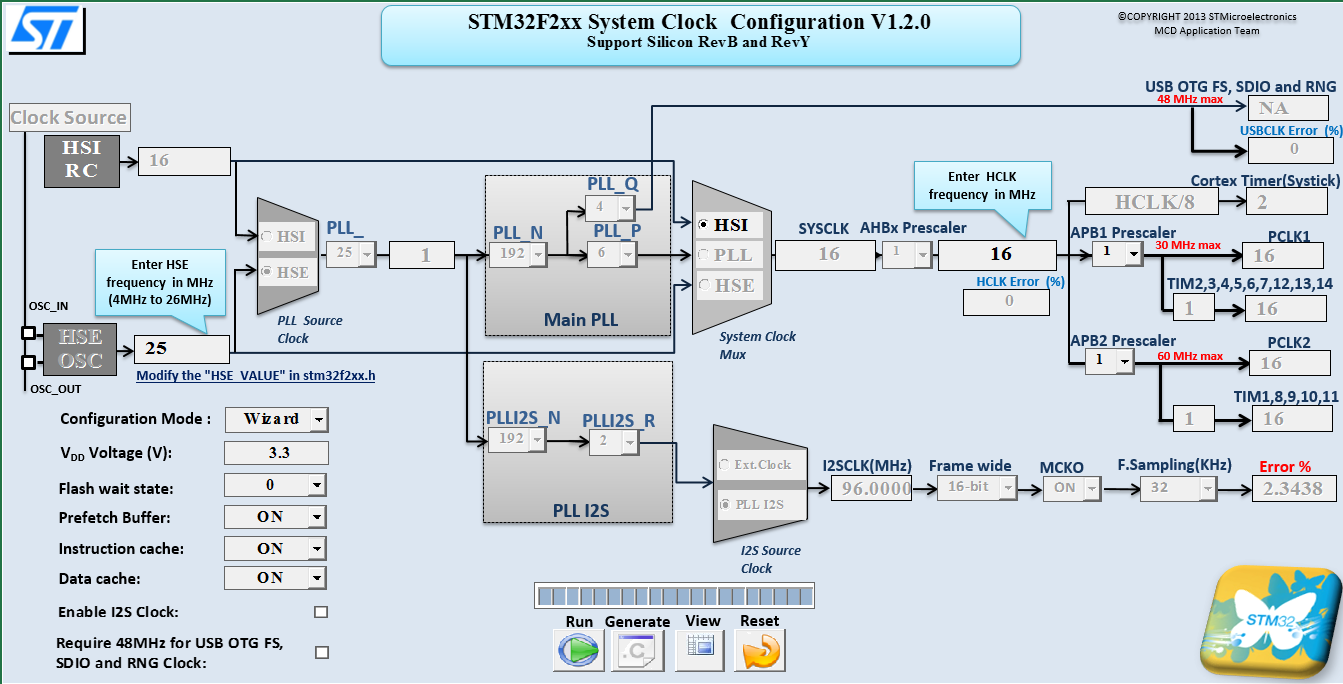
\includegraphics[width = \textwidth]{liczniki}
\caption{Schemat konfiguracji licznika}
\end{figure}

\end{center}
Konfiguracja wewnętrznych timerów została przeprowadzona za pomocą biblioteki HAL. Został wybrany 32-bitowy licznik zliczający przejścia zegara procesora z logicznego ,,0'' na ,,1''. W ten sposób uzyskany został pomiar z dokładnością do $\frac{1}{48000000}$ sekundy i maksymalną mierzoną wartością $2^{32} * \frac{1}{48000000} \approx$ 90 sekund. Do pomiaru czasu służą 3 proste funkcje: inicjalizująca timer, rozpoczynająca oraz kończąca pomiar.
\\Funkcja inicjująca najpierw wybiera timer2 (32-bitowy), ustawia preskaler oraz dzielnik częstotliwości na 1 aby osiągnąć maksymalną dokładność pomiaru oraz ustawia kierunek zliczania impulsów w górę i makysmalną wartość timera na 0xFFFFFFFF:\\
\texttt{
void TimerInit( TIM\_HandleTypeDef *timerHandle)\\
\{\\
\hspace*{10mm}timerHandle->Instance = TIM2;\\
\hspace*{10mm}\_\_TIM2\_CLK\_ENABLE();\\
\hspace*{10mm}timerHandle->Init.Prescaler = 1;\\
\hspace*{10mm}timerHandle->Init.CounterMode = TIM\_COUNTERMODE\_UP;\\
\hspace*{10mm}timerHandle->Init.Period = 0xFFFFFFFF;\\
\hspace*{10mm}timerHandle->Init.ClockDivision = 1;\\\}\\
}
\\Funkcja rozpoczynająca pomiar, wołana po inicjacji timera ustawia aktualną wartość zliczany impulsów:\\
\texttt{
void TimerStart(TIM\_HandleTypeDef *timerHandle)\\
\{\\
\hspace*{10mm}timerHandle->Instance->CNT = 0;\\
\}\\
}
\\Funkcja kończąca pomiar, wołana po inicjacji timera odczytuje aktualną ilość zliczonych impulsów i zwraca jej wartość:\\
\texttt{
uint32\_t TimerStop(TIM\_HandleTypeDef *timerHandle)\\
\{\\
\hspace*{10mm}return timerHandle->Instance->CNT;\\
\}
}
\chapter{Pomiary czasów poszczególnych algorytmów z biblioteki WolfSSL}

Poszczeólne algorytmy były wykonywane dla reprezentacyjnych danych testowych. Taktowanie zegara wynosiło 96 MHz. Przezntowane wyniki zawierają dane każdego z 30 testów jak i czasy średnich wykonań algorytmów.
\section{Algorytm SHA-1}

SHA-1 to powstały w 1993 roku algorytm hashujący. Jako dane wejściowe pobiera wiadomość o maksymalnej długości $2^{64}$ bitów i zamienia je w 160-bitowy skrót. Tak jak wszystkie algorytmy haszujące, głównym zastosowaniem algorytmu SHA-1 jest weryfikacja inegralności plików lub wiadomości. Wraz z każdą wiadomością może być wysyłany jej skrót SHA-1. W momencie gdy adresat odbiera wiadomość oblicza jej skrót SHA-1. Jeżeli skróty są od siebie różne, to mamy pewność że któryś z bitów został źle odebrany i wiadomość nie może dalej być przetwarzana. Niestety w 2005 roku zostały opublikowane pierwsze ataki pozwalające złamać skrót w czasie krótszym niż atakiem typu BruteForce (sprawdzanie każdej możlwiości po kolei) i używanie tego algorytmu hashującego w nowych systemach nie jest zalecane. 

\subsection{Software'owa implementacja algorytmu}

Algorytm SHA-1 składa się z trzech części: inicjalizacja danych, przetwarzanie wszystkich danych poza ostatnią częsią, przetworzenie ostatniej części. Dane przetwarzane są partiami po 32 bajty w każdym cyklu. W każdym cyklu na bajtach dokonywane są operacje logiczne: and i xor, a także operacja przesuwania bitowego. Dokładny opis algorytmu znajduje się w Dodatku A.\\
Badania przeprowadzono dla 30 wywołań algorytmu dla danych testowych o długościach: 32 bajtów, 64 bajtów i 1 kilobajta. Wyniki są dostępne na kolejnej stronie:


\begin{table}[!h]

\centering
\begin{adjustwidth}{-1cm}{}
\newcolumntype{C}{>{\centering\arraybackslash}X}%
        \begin{tabularx}{18 cm}{|C|C|C|C|C|C|C|C|C|C|}
        \hline 
         & \multicolumn{3}{|c|}{32 bajty} & \multicolumn{3}{|c|}{64 bajty} & \multicolumn{3}{|c|}{1024 bajty} \\
        \cline{2-10}
{\fontsize{10}{12}\selectfont Nr} & {\fontsize{10}{12}\selectfont licznik} &  {\fontsize{10}{12}\selectfont czas [ms]} & {\fontsize{10}{12}\selectfont prędkość [MB/s]} & {\fontsize{10}{12}\selectfont licznik} & {\fontsize{10}{12}\selectfont czas [ms]} &{\fontsize{10}{12}\selectfont prędkość [MB/s]} & {\fontsize{10}{12}\selectfont licznik} &{\fontsize{10}{12}\selectfont czas [ms]} &{\fontsize{10}{12}\selectfont prędkość [MB/s]} \\
            \hline
1	& 690 &	0.014 &	2.226 &	1261 &	0.026 &	2.436 &	10004 &	0.208 &	4.913 \\
\hline
2 &	691	& 0.014	& 2.223 &	1261 &	0.026 &	2.436 &	10015 &	0.209 &	4.908 \\ \hline
3 &	691	& 0.014	& 2.223 &	1261 &	0.026 &	2.436 &	10004 &	0.208 &	4.913 \\ \hline
4 &	690	& 0.014	& 2.226 &	1260 &	0.026 &	2.438 &	10015 &	0.209 &	4.908 \\ \hline
5 &	691	& 0.014	& 2.223 &	1261 &	0.026 &	2.436 &	10005 &	0.208 &	4.913 \\ \hline
6 &	690	& 0.014	& 2.226 &	1261 &	0.026 &	2.436 &	10014 &	0.209 &	4.908 \\ \hline
7 &	690	& 0.014	& 2.226 &	1260 &	0.026 &	2.438 &	10005 &	0.208 &	4.913 \\ \hline
8 &	690	& 0.014	& 2.226 &	1260 &	0.026 &	2.438 &	10015 &	0.209 &	4.908 \\ \hline
9 &	691	& 0.014	& 2.223 &	1261 &	0.026 &	2.436 &	10004 &	0.208 &	4.913 \\ \hline
10 &	690	& 0.014 &	2.226 &	1260 &	0.026 &	2.438 &	10015 &	0.209 &	4.908 \\ \hline
11 &	690	& 0.014 &	2.226 &	1260 &	0.026 &	2.438 &	10004 &	0.208 &	4.913 \\ \hline
12 &	690	& 0.014 &	2.226 &	1261 &	0.026 &	2.436 &	10015 &	0.209 &	4.908 \\ \hline
13 &	691	& 0.014 &	2.223 &	1260 &	0.026 &	2.438 &	10004 &	0.208 &	4.913 \\ \hline
14 &	691	& 0.014 &	2.223 &	1260 &	0.026 &	2.438 &	10014 &	0.209 &	4.908 \\ \hline
15 &	691	& 0.014 &	2.223 &	1260 &	0.026 &	2.438 &	10005 &	0.208 &	4.913 \\ \hline
16 &	691	& 0.014 &	2.223 &	1260 &	0.026 &	2.438 &	10015 &	0.209 &	4.908 \\ \hline
17 &	690	& 0.014 &	2.226 &	1261 &	0.026 &	2.436 &	10005 &	0.208 &	4.913 \\ \hline
18 &	690	& 0.014 &	2.226 &	1260 &	0.026 &	2.438 &	10015 &	0.209 &	4.908 \\ \hline
19 &	690	& 0.014 &	2.226 &	1271 &	0.026 &	2.417 &	10005 &	0.208 &	4.913 \\ \hline
20 &	691	& 0.014 &	2.223 &	1260 &	0.026 &	2.438 &	10015 &	0.209 &	4.908 \\ \hline
21 &	691	& 0.014 &	2.223 &	1260 &	0.026 &	2.438 &	10005 &	0.208 &	4.913 \\ \hline
22 &	690	& 0.014 &	2.226 &	1260 &	0.026 &	2.438 &	10015 &	0.209 &	4.908 \\ \hline
23 &	690	& 0.014 &	2.226 &	1260 &	0.026 &	2.438 &	10005 &	0.208 &	4.913 \\ \hline
24 &	690	& 0.014 &	2.226 &	1260 &	0.026 &	2.438 &	10016 &	0.209 &	4.907 \\ \hline
25 &	690	& 0.014 &	2.226 &	1261 &	0.026 &	2.436 &	10004 &	0.208 &	4.913 \\ \hline
26 &	690	& 0.014 &	2.226 &	1260 &	0.026 &	2.438 &	10016 &	0.209 &	4.907 \\ \hline
27 &	690	& 0.014 &	2.226 &	1263 &	0.026 &	2.432 &	10004 &	0.208 &	4.913 \\ \hline
28 &	690	& 0.014 &	2.226 &	1261 &	0.026 &	2.436 &	10007 &	0.208 &	4.912 \\ \hline
29 &	690	& 0.014 &	2.226 &	1260 &	0.026 &	2.438 &	10004 &	0.208 &	4.913 \\ \hline
30 &	690	& 0.014 &	2.226 &	1260 &	0.026 &	2.438 &	10016 &	0.209 &	4.907 \\ \hline
\textbf{Średnia}	& \textbf{690} &	\textbf{0.014} &	\textbf{2.225} &	\textbf{1261} &	\textbf{0.026} &	\textbf{2.437} &	\textbf{10010} &	\textbf{0.209} & \textbf{4.911} \\ \hline
    \end{tabularx}
    \caption{Czasy dla algorytmu SHA-1}
        \end{adjustwidth}
\end{table}
\subsection{Hardware'owa implementacja algorytmu}

Użyty procesor STM32f217IGH6 posiada specjalnie dedykowane kryptoprocesory do wykonania algorytmu SHA-1. Można się do niego dostać dzięki bibliotece STM32F2xx\_StdPeriph\_Driver, a konkretnie interfejsowi hardware'owemu dostępnemu w pliku stm32f2xx\_hash.c. Posiada on funkcje, które obsługują krpytoprocesor i biblioteka WolfSSL z nich korzysta. Czasy uzyskane przy pomocy wsparcia hardware'owego dla tych samych danych testowych są na kolejenj stronie.

\begin{table}

\centering
\begin{adjustwidth}{-1cm}{}
\newcolumntype{C}{>{\centering\arraybackslash}X}%
        \begin{tabularx}{18 cm}{|C|C|C|C|C|C|C|C|C|C|}
        \hline 
         & \multicolumn{3}{|c|}{32 bajty} & \multicolumn{3}{|c|}{64 bajty} & \multicolumn{3}{|c|}{1024 bajty} \\
        \cline{2-10}
{\fontsize{10}{12}\selectfont Nr} & {\fontsize{10}{12}\selectfont licznik} &  {\fontsize{10}{12}\selectfont czas [ms]} & {\fontsize{10}{12}\selectfont prędkość [MB/s]} & {\fontsize{10}{12}\selectfont licznik} & {\fontsize{10}{12}\selectfont czas [ms]} &{\fontsize{10}{12}\selectfont prędkość [MB/s]} & {\fontsize{10}{12}\selectfont licznik} &{\fontsize{10}{12}\selectfont czas [ms]} &{\fontsize{10}{12}\selectfont prędkość [MB/s]} \\
            \hline
1	& 254 &	0.005 &	6.047 &	318 &	0.007 &	9.660 &	2282 &	0.048 &	21.539 \\ \hline
2	& 253 &	0.005 &	6.071 &	318 &	0.007 &	9.660 &	2292 &	0.048 &	21.445 \\ \hline
3	& 254 &	0.005 &	6.047 &	318 &	0.007 &	9.660 &	2282 &	0.048 &	21.539 \\ \hline
4	& 254 &	0.005 &	6.047 &	317 &	0.007 &	9.691 &	2282 &	0.048 &	21.539 \\ \hline
5	& 254 &	0.005 &	6.047 &	318 &	0.007 &	9.660 &	2282 &	0.048 &	21.539 \\ \hline
6	& 253 &	0.005 &	6.071 &	318 &	0.007 &	9.660 &	2282 &	0.048 &	21.539 \\ \hline
7	& 253 &	0.005 &	6.071 &	317 &	0.007 &	9.691 &	2282 &	0.048 &	21.539 \\ \hline
8	& 253 &	0.005 &	6.071 &	317 &	0.007 &	9.691 &	2282 &	0.048 &	21.539 \\ \hline
9	& 254 &	0.005 &	6.047 &	317 &	0.007 &	9.691 &	2282 &	0.048 &	21.539 \\ \hline
10 &	254	& 0.005	& 6.047	& 317	& 0.007 &	9.691 &	2282 &	0.048 &	21.539 \\ \hline
11 &	253	& 0.005	& 6.071	& 317	& 0.007 &	9.691 &	2282 &	0.048 &	21.539 \\ \hline
12 &	253	& 0.005	& 6.071	& 317	& 0.007 &	9.691 &	2282 &	0.048 &	21.539 \\ \hline
13 &	253	& 0.005	& 6.071	& 318	& 0.007 &	9.660 &	2282 &	0.048 &	21.539 \\ \hline
14 &	253	& 0.005	& 6.071	& 317	& 0.007 &	9.691 &	2282 &	0.048 &	21.539 \\ \hline
15 &	254	& 0.005	& 6.047	& 317	& 0.007 &	9.691 &	2282 &	0.048 &	21.539 \\ \hline
16 &	254	& 0.005	& 6.047	& 317	& 0.007 &	9.691 &	2282 &	0.048 &	21.539 \\ \hline
17 &	254	& 0.005	& 6.047	& 318	& 0.007 &	9.660 &	2282 &	0.048 &	21.539 \\ \hline
18 &	254	& 0.005	& 6.047	& 317	& 0.007 &	9.691 &	2282 &	0.048 &	21.539 \\ \hline
19 &	253	& 0.005	& 6.071	& 318	& 0.007 &	9.660 &	2282 &	0.048 &	21.539 \\ \hline
20 &	253	& 0.005	& 6.071	& 317	& 0.007 &	9.691 &	2282 &	0.048 &	21.539 \\ \hline
21 &	254	& 0.005	& 6.047	& 317	& 0.007 &	9.691 &	2292 &	0.048 &	21.445 \\ \hline
22 &	254	& 0.005	& 6.047	& 318	& 0.007 &	9.660 &	2282 &	0.048 &	21.539 \\ \hline
23 &	254	& 0.005	& 6.047	& 317	& 0.007 &	9.691 &	2282 &	0.048 &	21.539 \\ \hline
24 &	254	& 0.005	& 6.047	& 317	& 0.007 &	9.691 &	2282 &	0.048 &	21.539 \\ \hline
25 &	254	& 0.005	& 6.047	& 317	& 0.007 &	9.691 &	2282 &	0.048 &	21.539 \\ \hline
26 &	253	& 0.005	& 6.071	& 318	& 0.007 &	9.660 &	2282 &	0.048 &	21.539 \\ \hline
27 &	254	& 0.005	& 6.047	& 317	& 0.007 &	9.691 &	2282 &	0.048 &	21.539 \\ \hline
28 &	254	& 0.005	& 6.047	& 318	& 0.007 &	9.660 &	2282 &	0.048 &	21.539 \\ \hline
29 &	254	& 0.005	& 6.047	& 318	& 0.007 &	9.660 &	2282 &	0.048 &	21.539 \\ \hline
30 &	254	& 0.005	& 6.047	& 318	& 0.007 &	9.660 &	2282 &	0.048 &	21.539 \\ \hline
\textbf{Średnia} &	\textbf{254} &	0.\textbf{005} &	\textbf{6.056} &	\textbf{317}	& \textbf{0.007}	& \textbf{9.678}	& \textbf{2283}	& \textbf{0.048}	& \textbf{21.533} \\ \hline


    \end{tabularx}
    \caption{Czasy dla algorytmu SHA-1 ze wsparciem sprzętowym}
        \end{adjustwidth}
\end{table}\pagebreak 

\section{Algorytm DES}
Algorytm DES (eng. Data Encryption Standard) jest symetrycznym szyfrem blokowym zapoczątkowanym przez IBM w 1975 r. Algorytm mając klucz i wektor inicjujący zamienia 8 bajtów wejściowych w 8 bajtów wyjściowych, które mogą następnie być z powrotem odszydrowane o ile adresat zna klucz użyty do zaszyfrowania wiadomości. Z matematycznego punktu widzenia DES jest funkcją różnowartościową która każdej wartości z dziedziny funkcji $D \in \left( 0, 2^{64}-1 \right)$ przypisuje jedną wartość z jej przeciwdziedziny $Y \in \left( 0, 2^{64}-1 \right)$.\\
Z uwagi na małą długość klucza - tylko 56 bitów algorytm ten uznawany jest za podatny na ataki typu brute force.
\subsection{Software'owa implementacja algorytmu}
Pierwszym krokiem jest generowanie 16 rund kluczy na podstawie jednego klucza głównego. Następnie algorytm przetwarza dane w 8-bajtowych porcjach. Każda porcja jest podawana operacjom matematycznym takim jak permutacja bitów, operacja bitowa xor, dokonywanie podstawień na podstawie S-boxy i P-boxy (są to takie ,,czarne skrzynki'' które zamieniają liczby S-box z liczby z zakresu 0-63 na liczbę z zakresu 0-15, a P-box z 0-31 na liczbę 0-31, oraz funcje Feistela.\\Dokładny opis algorytmu znajduje się w dodatku B. Czasy szyfrowania danych z użyciem algorytmu DES przedstawia tabela na kolejnej stronie.
\begin{table}

\centering
\begin{adjustwidth}{-1cm}{}
\newcolumntype{C}{>{\centering\arraybackslash}X}%
        \begin{tabularx}{18 cm}{|C|C|C|C|C|C|C|C|C|C|C|C|}
        \hline 
         & \multicolumn{2}{|c|}{Generowanie kluczy} & \multicolumn{3}{|c|}{8 bajtów} & \multicolumn{3}{|c|}{16 bajtów} & \multicolumn{3}{|c|}{1024 bajty} \\
        \cline{2-12}
{\fontsize{10}{12}\selectfont Nr} & {\fontsize{10}{12}\selectfont licznik} &  {\fontsize{10}{12}\selectfont czas [ms]} & {\fontsize{10}{12}\selectfont licznik} &  {\fontsize{10}{12}\selectfont czas [ms]}& {\fontsize{10}{12}\selectfont prędkość [MB/s]} & {\fontsize{10}{12}\selectfont licznik} & {\fontsize{10}{12}\selectfont czas [ms]} &{\fontsize{10}{12}\selectfont prędkość [MB/s]} & {\fontsize{10}{12}\selectfont licznik} &{\fontsize{10}{12}\selectfont czas [ms]} &{\fontsize{10}{12}\selectfont prędkość [MB/s]} \\
            \hline
1 &	10155 &	0.212 &	434 &	0.009 &	0.885 &	843 &	0.018 &	0.911 &	52261 &	1.089 &	0.941 \\ \hline
2 &	10155 &	0.212 &	435 &	0.009 &	0.883 &	844 &	0.018 &	0.910 &	52260 &	1.089 &	0.941 \\ \hline
3 &	10155 &	0.212 &	435 &	0.009 &	0.883 &	844 &	0.018 &	0.910 &	52261 &	1.089 &	0.941 \\ \hline
4 &	10155 &	0.212 &	435 &	0.009 &	0.883 &	844 &	0.018 &	0.910 &	52261 &	1.089 &	0.941 \\ \hline
5 &	10155 &	0.212 &	435 &	0.009 &	0.883 &	844 &	0.018 &	0.910 &	52260 &	1.089 &	0.941 \\ \hline
6 &	10155 &	0.212 &	435 &	0.009 &	0.883 &	844 &	0.018 &	0.910 &	52260 &	1.089 &	0.941 \\ \hline
7 &	10155 &	0.212 &	435 &	0.009 &	0.883 &	844 &	0.018 &	0.910 &	52262 &	1.089 &	0.940 \\  \hline
8 &	10155 &	0.212 &	435 &	0.009 &	0.883 &	844 &	0.018 &	0.910 &	52260 &	1.089 &	0.941 \\  \hline
9 &	10165 &	0.212 &	435 &	0.009 &	0.883 &	844 &	0.018 &	0.910 &	52261 &	1.089 &	0.941 \\  \hline
10 &	10155 &	0.212 &	435 &	0.009 &	0.883 &	855 &	0.018 &	0.898 &	52260 &	1.089 &	0.941 \\  \hline
11 &	10167 &	0.212 &	435 &	0.009 &	0.883 &	844 &	0.018 &	0.910 &	52260 &	1.089 &	0.941 \\  \hline
12 &	10155 &	0.212 &	435 &	0.009 &	0.883 &	843 &	0.018 &	0.911 &	52260 &	1.089 &	0.941 \\  \hline
13 &	10166 &	0.212 &	435 &	0.009 &	0.883 &	844 &	0.018 &	0.910 &	52261 &	1.089 &	0.941 \\  \hline
14 &	10155 &	0.212 &	435 &	0.009 &	0.883 &	844 &	0.018 &	0.910 &	52261 &	1.089 &	0.941 \\  \hline
15 &	10166 &	0.212 &	435 &	0.009 &	0.883 &	844 &	0.018 &	0.910 &	52262 &	1.089 &	0.940 \\  \hline
16 &	10155 &	0.212 &	435 &	0.009 &	0.883 &	844 &	0.018 &	0.910 &	52260 &	1.089 &	0.941 \\  \hline
17 &	10168 &	0.212 &	435 &	0.009 &	0.883 &	844 &	0.018 &	0.910 &	52261 &	1.089 &	0.941 \\  \hline
18 &	10155 &	0.212 &	435 &	0.009 &	0.883 &	844 &	0.018 &	0.910 &	52262 &	1.089 &	0.940 \\  \hline
19 &	10169 &	0.212 &	435 &	0.009 &	0.883 &	844 &	0.018 &	0.910 &	52260 &	1.089 &	0.941 \\  \hline
20 &	10155 &	0.212 &	435 &	0.009 &	0.883 &	844 &	0.018 &	0.910 &	52260 &	1.089 &	0.941 \\  \hline
21 &	10169 &	0.212 &	435 &	0.009 &	0.883 &	844 &	0.018 &	0.910 &	52272 &	1.089 &	0.940 \\  \hline
22 &	10155 &	0.212 &	435 &	0.009 &	0.883 &	844 &	0.018 &	0.910 &	52261 &	1.089 &	0.941 \\  \hline
23 &	10168 &	0.212 &	435 &	0.009 &	0.883 &	844 &	0.018 &	0.910 &	52261 &	1.089 &	0.941 \\  \hline
24 &	10155 &	0.212 &	435 &	0.009 &	0.883 &	844 &	0.018 &	0.910 &	52273 &	1.089 &	0.940 \\  \hline
25 &	10169 &	0.212 &	435 &	0.009 &	0.883 &	844 &	0.018 &	0.910 &	52260 &	1.089 &	0.941 \\  \hline
26 &	10155 &	0.212 &	435 &	0.009 &	0.883 &	844 &	0.018 &	0.910 &	52260 &	1.089 &	0.941 \\  \hline
27 &	10168 &	0.212 &	435 &	0.009 &	0.883 &	844 &	0.018 &	0.910 &	52271 &	1.089 &	0.940 \\  \hline
28 &	10155 &	0.212 &	435 &	0.009 &	0.883 &	844 &	0.018 &	0.910 &	52261 &	1.089 &	0.941 \\  \hline
29 &	10167 &	0.212 &	435 &	0.009 &	0.883 &	844 &	0.018 &	0.910 &	52261 &	1.089 &	0.941 \\  \hline
30 &	10155 &	0.212 &	435 &	0.009 &	0.883 &	844 &	0.018 &	0.910 &	52271 &	1.089 &	0.940 \\  \hline
\textbf{Średnia}	 &\textbf{10160}	 &\textbf{0.212}	 &\textbf{435}	 &\textbf{0.0091} &	\textbf{0.883} &	\textbf{844} &	\textbf{0.018} &	\textbf{0.910} &	\textbf{52262} &	\textbf{1.089} &	\textbf{0.940} \\  \hline

    \end{tabularx}
    \caption{Czasy dla algorytmu DES}
        \end{adjustwidth}
\end{table}

\subsection{Hardware'owa implementacja algorytum}

Podobnie jak w przypadku SHA-1 także DES posiada swój koprocesor kryptograficzny na pokładzie STM32f217IGH6. Dzięki zastosowaniu funkcji znajdujących się w plikach stm32f2xx\_cryp.c i stm32f2xx\_cryp\_des.c uzyskujemy interfejs pozwalający na korzystanie z koprocesora. Biblioteka WolfSSL oferuje wsparcie dla koprocesora (przez ustawienie flagi STM32\_CRYPT przy kompilacji) co pozwala na znaczące przyspieszenie wykonywanych obliczeń. Wyniki pomiarów czasu zaprezentowano w tablei na kolejnej stronie.
\begin{table}

\centering
\begin{adjustwidth}{-1cm}{}
\newcolumntype{C}{>{\centering\arraybackslash}X}%
        \begin{tabularx}{18 cm}{|C|C|C|C|C|C|C|C|C|C|C|C|}
        \hline 
         & \multicolumn{2}{|c|}{Generowanie kluczy} & \multicolumn{3}{|c|}{8 bajtów} & \multicolumn{3}{|c|}{16 bajtów} & \multicolumn{3}{|c|}{1024 bajty} \\
        \cline{2-12}
{\fontsize{10}{12}\selectfont Nr} & {\fontsize{10}{12}\selectfont licznik} &  {\fontsize{10}{12}\selectfont czas [ms]} & {\fontsize{10}{12}\selectfont licznik} &  {\fontsize{10}{12}\selectfont czas [ms]}& {\fontsize{10}{12}\selectfont prędkość [MB/s]} & {\fontsize{10}{12}\selectfont licznik} & {\fontsize{10}{12}\selectfont czas [ms]} &{\fontsize{10}{12}\selectfont prędkość [MB/s]} & {\fontsize{10}{12}\selectfont licznik} &{\fontsize{10}{12}\selectfont czas [ms]} &{\fontsize{10}{12}\selectfont prędkość [MB/s]} \\
            \hline
1 &	34 &	0.001 &	250 &	0.005 &	1.536 &	298 &	0.006 &	2.577 &	6220 &	0.130 &	7.902 \\ \hline
2 &	34	& 0.001	& 251	& 0.005 &	1.530 &	298 &	0.006 &	2.577 &	6230 &	0.130 &	7.890 \\ \hline
3 &	34	& 0.001	& 251	& 0.005 &	1.530 &	298 &	0.006 &	2.577 &	6219 &	0.130 &	7.904 \\ \hline
4 &	34	& 0.001	& 251	& 0.005 &	1.530 &	298 &	0.006 &	2.577 &	6219 &	0.130 &	7.904 \\ \hline
5 &	34	& 0.001	& 251	& 0.005 &	1.530 &	309 &	0.006 &	2.485 &	6230 &	0.130 &	7.890 \\ \hline
6 &	34	& 0.001	& 251	& 0.005 &	1.530 &	298 &	0.006 &	2.577 &	6219 &	0.130 &	7.904 \\ \hline
7 &	34	& 0.001	& 251	& 0.005 &	1.530 &	298 &	0.006 &	2.577 &	6219 &	0.130 &	7.904 \\ \hline
8 &	34	& 0.001	& 251	& 0.005 &	1.530 &	298 &	0.006 &	2.577 &	6219 &	0.130 &	7.904 \\ \hline
9 &	34	& 0.001	& 251	& 0.005 &	1.530 &	298 &	0.006 &	2.577 &	6229 &	0.130 &	7.891 \\ \hline
10 &	34	& 0.001	& 251	& 0.005 &	1.530 &	298 &	0.006 &	2.577 &	6219 &	0.130 &	7.904 \\ \hline
11 &	34	& 0.001	& 251	& 0.005 &	1.530 &	298 &	0.006 &	2.577 &	6219 &	0.130 &	7.904 \\ \hline
12 &	34	& 0.001	& 251	& 0.005 &	1.530 &	298 &	0.006 &	2.577 &	6230 &	0.130 &	7.890 \\ \hline
13 &	34	& 0.001	& 251	& 0.005 &	1.530 &	298 &	0.006 &	2.577 &	6219 &	0.130 &	7.904 \\ \hline
14 &	34	& 0.001	& 251	& 0.005 &	1.530 &	298 &	0.006 &	2.577 &	6219 &	0.130 &	7.904 \\ \hline
15 &	34	& 0.001	& 251	& 0.005 &	1.530 &	298 &	0.006 &	2.577 &	6230 &	0.130 &	7.890 \\ \hline
16 &	34	& 0.001	& 251	& 0.005 &	1.530 &	298 &	0.006 &	2.577 &	6219 &	0.130 &	7.904 \\ \hline
17 &	34	& 0.001	& 251	& 0.005 &	1.530 &	298 &	0.006 &	2.577 &	6219 &	0.130 &	7.904 \\ \hline
18 &	34	& 0.001	& 251	& 0.005 &	1.530 &	298 &	0.006 &	2.577 &	6230 &	0.130 &	7.890 \\ \hline
19 &	34	& 0.001	& 251	& 0.005 &	1.530 &	298 &	0.006 &	2.577 &	6219 &	0.130 &	7.904 \\ \hline
20 &	34	& 0.001	& 251	& 0.005 &	1.530 &	298 &	0.006 &	2.577 &	6219 &	0.130 &	7.904 \\ \hline
21 &	34	& 0.001	& 251	& 0.005 &	1.530 &	298 &	0.006 &	2.577 &	6219 &	0.130 &	7.904 \\ \hline
22 &	34	& 0.001	& 251	& 0.005 &	1.530 &	309 &	0.006 &	2.485 &	6220 &	0.130 &	7.902 \\ \hline
23 &	34	& 0.001	& 251	& 0.005 &	1.530 &	298 &	0.006 &	2.577 &	6219 &	0.130 &	7.904 \\ \hline
24 &	34	& 0.001	& 251	& 0.005 &	1.530 &	298 &	0.006 &	2.577 &	6219 &	0.130 &	7.904 \\ \hline
25 &	34	& 0.001	& 251	& 0.005 &	1.530 &	298 &	0.006 &	2.577 &	6230 &	0.130 &	7.890 \\ \hline
26 &	34	& 0.001	& 251	& 0.005 &	1.530 &	298 &	0.006 &	2.577 &	6219 &	0.130 &	7.904 \\ \hline
27 &	34	& 0.001	& 251	& 0.005 &	1.530 &	298 &	0.006 &	2.577 &	6219 &	0.130 &	7.904 \\ \hline
28 &	34	& 0.001	& 251	& 0.005 &	1.530 &	298 &	0.006 &	2.577 &	6230 &	0.130 &	7.890 \\ \hline
29 &	34	& 0.001	& 251	& 0.005 &	1.530 &	298 &	0.006 &	2.577 &	6219 &	0.130 &	7.904 \\ \hline
30 &	34	& 0.001	& 251	& 0.005 &	1.530 &	298 &	0.006 &	2.577 &	6219 &	0.130 &	7.904 \\ \hline
\textbf{Średnia} &	\textbf{34}	& \textbf{0.001}	& \textbf{251}	& \textbf{0.005} &	\textbf{1.530} &	\textbf{299} &	\textbf{0.006} &	\textbf{2.571} &	\textbf{6222} &	\textbf{0.130} &	\textbf{7.900} \\ \hline



    \end{tabularx}
    \caption{Czasy dla algorytmu DES ze wsparciem sprzętowym}
    \end{adjustwidth}
\end{table} \pagebreak

\section{Algorytm AES}
AES (eng. Advanced Encryption Standard) jest symetrycznym szyfrem blokowym, który przetwarza dane w paczkach po 16 bajtów każda. Podobnie jak DES też składa się z części obliczającej klucze rundy i z części kodującej wiadomość. Algorytm jest uznawany za bezpieczny i jest zalecany zamiast algorytmu DES, który przez krótki klucz jest łatwy do złamania.\\


\subsection{Software'owa wydajność algorytmu}
Pierwszym krokiem jest wygenerowanie kluczy 11/13/15 kluczy rund, następnie dane są kodowane w 10/12/14 rundach (pierwszy klucz dodawany jest na samym początku). Na danych dokonywane są takie operacje jak logiczny xor, cykliczne obracanie bajtów/bitów, podstawianie bajtów. Dokładny opis algorytmu przedstawiony jest w dodatku C. Czasy szyfrowania danych z użyciem algorytmu AES przedstawaiają tabele na kolejnych stronach.

\begin{table}
\begin{adjustwidth}{-1cm}{}
\centering
\newcolumntype{C}{>{\centering\arraybackslash}X}%

        \begin{tabularx}{18 cm}{|C|C|C|C|C|C|C|C|C|C|C|C|}
        \hline 
         & \multicolumn{2}{|c|}{Generowanie kluczy} & \multicolumn{3}{|c|}{16 bajtów} & \multicolumn{3}{|c|}{32 bajtów} & \multicolumn{3}{|c|}{1024 bajty} \\
        \cline{2-12}
{\fontsize{10}{12}\selectfont Nr} & {\fontsize{10}{12}\selectfont licznik} &  {\fontsize{10}{12}\selectfont czas [ms]} & {\fontsize{10}{12}\selectfont licznik} &  {\fontsize{10}{12}\selectfont czas [ms]}& {\fontsize{10}{12}\selectfont prędkość [MB/s]} & {\fontsize{10}{12}\selectfont licznik} & {\fontsize{10}{12}\selectfont czas [ms]} &{\fontsize{10}{12}\selectfont prędkość [MB/s]} & {\fontsize{10}{12}\selectfont licznik} &{\fontsize{10}{12}\selectfont czas [ms]} &{\fontsize{10}{12}\selectfont prędkość [MB/s]} \\
            \hline
1 &	260 &	0.0054 &	461 &	0.0096 &	1.666 &	890 &	0.019 &	1.726 &	27645 &	0.576 &	1.778 \\ \hline
2 &	260 &	0.0054 &	462 &	0.0096 &	1.662 &	890 &	0.019 &	1.726 &	27645 &	0.576 &	1.778 \\ \hline
3 &	261 &	0.0054 &	462 &	0.0096 &	1.662 &	890 &	0.019 &	1.726 &	27647 &	0.576 &	1.778 \\ \hline
4 &	260 &	0.0054 &	462 &	0.0096 &	1.662 &	890 &	0.019 &	1.726 &	27656 &	0.576 &	1.777 \\ \hline
5 &	260 &	0.0054 &	462 &	0.0096 &	1.662 &	890 &	0.019 &	1.726 &	27646 &	0.576 &	1.778 \\ \hline
6 &	260 &	0.0054 &	462 &	0.0096 &	1.662 &	890 &	0.019 &	1.726 &	27645 &	0.576 &	1.778 \\ \hline
7 &	260 &	0.0054 &	462 &	0.0096 &	1.662 &	900 &	0.019 &	1.707 &	27645 &	0.576 &	1.778 \\ \hline
8 &	260 &	0.0054 &	462 &	0.0096 &	1.662 &	890 &	0.019 &	1.726 &	27645 &	0.576 &	1.778 \\ \hline
9 &	260 &	0.0054 &	462 &	0.0096 &	1.662 &	890 &	0.019 &	1.726 &	27646 &	0.576 &	1.778 \\ \hline
10 &	260 &	0.0054 &	462 &	0.0096 &	1.662 &	890 &	0.019 &	1.726 &	27645 &	0.576 &	1.778 \\ \hline
11 &	260 &	0.0054 &	462 &	0.0096 &	1.662 &	890 &	0.019 &	1.726 &	27646 &	0.576 &	1.778 \\ \hline
12 &	260 &	0.0054 &	462 &	0.0096 &	1.662 &	890 &	0.019 &	1.726 &	27645 &	0.576 &	1.778 \\ \hline
13 &	260 &	0.0054 &	461 &	0.0096 &	1.666 &	890 &	0.019 &	1.726 &	27657 &	0.576 &	1.777 \\ \hline
14 &	260 &	0.0054 &	462 &	0.0096 &	1.662 &	890 &	0.019 &	1.726 &	27645 &	0.576 &	1.778 \\ \hline
15 &	260 &	0.0054 &	462 &	0.0096 &	1.662 &	890 &	0.019 &	1.726 &	27646 &	0.576 &	1.778 \\ \hline
16 &	260 &	0.0054 &	462 &	0.0096 &	1.662 &	890 &	0.019 &	1.726 &	27646 &	0.576 &	1.778 \\ \hline
17 &	260 &	0.0054 &	462 &	0.0096 &	1.662 &	890 &	0.019 &	1.726 &	27645 &	0.576 &	1.778 \\ \hline
18 &	260 &	0.0054 &	462 &	0.0096 &	1.662 &	890 &	0.019 &	1.726 &	27646 &	0.576 &	1.778 \\ \hline
19 &	260 &	0.0054 &	462 &	0.0096 &	1.662 &	890 &	0.019 &	1.726 &	27647 &	0.576 &	1.778 \\ \hline
20 &	260 &	0.0054 &	462 &	0.0096 &	1.662 &	890 &	0.019 &	1.726 &	27646 &	0.576 &	1.778 \\ \hline
21 &	261 &	0.0054 &	462 &	0.0096 &	1.662 &	890 &	0.019 &	1.726 &	27646 &	0.576 &	1.778 \\ \hline
22 &	260 &	0.0054 &	462 &	0.0096 &	1.662 &	890 &	0.019 &	1.726 &	27656 &	0.576 &	1.777 \\ \hline
23 &	260 &	0.0054 &	462 &	0.0096 &	1.662 &	890 &	0.019 &	1.726 &	27645 &	0.576 &	1.778 \\ \hline
24 &	260 &	0.0054 &	462 &	0.0096 &	1.662 &	890 &	0.019 &	1.726 &	27645 &	0.576 &	1.778 \\ \hline
25 &	260 &	0.0054 &	462 &	0.0096 &	1.662 &	890 &	0.019 &	1.726 &	27646 &	0.576 &	1.778 \\ \hline
26 &	260 &	0.0054 &	462 &	0.0096 &	1.662 &	890 &	0.019 &	1.726 &	27646 &	0.576 &	1.778 \\ \hline
27 &	260 &	0.0054 &	462 &	0.0096 &	1.662 &	890 &	0.019 &	1.726 &	27657 &	0.576 &	1.777 \\ \hline
28 &	260 &	0.0054 &	462 &	0.0096 &	1.662 &	890 &	0.019 &	1.726 &	27645 &	0.576 &	1.778 \\ \hline
29 &	260 &	0.0054 &	462 &	0.0096 &	1.662 &	890 &	0.019 &	1.726 &	27645 &	0.576 &	1.778 \\ \hline
30 &	260 &	0.0054 &	462 &	0.0096 &	1.662 &	890 &	0.019 &	1.726 &	27646 &	0.576 &	1.778 \\ \hline
\textbf{Średnia} &	\textbf{260} &	\textbf{0.0054} &	\textbf{462} &	\textbf{0.0096} &	\textbf{1.663} &	\textbf{890} &	\textbf{0.019} &	\textbf{1.725} &	\textbf{27647} &	\textbf{0.576} &	\textbf{1.778} \\ \hline


    \end{tabularx}
    \caption{Czasy dla algorytmu AES dla 10-ciu rund}
     \end{adjustwidth}
\end{table}

\begin{table}
\begin{adjustwidth}{-1cm}{}
\centering
\newcolumntype{C}{>{\centering\arraybackslash}X}%

        \begin{tabularx}{18 cm}{|C|C|C|C|C|C|C|C|C|C|C|C|}
        \hline 
         & \multicolumn{2}{|c|}{Generowanie kluczy} & \multicolumn{3}{|c|}{16 bajtów} & \multicolumn{3}{|c|}{32 bajtów} & \multicolumn{3}{|c|}{1024 bajty} \\
        \cline{2-12}
{\fontsize{10}{12}\selectfont Nr} & {\fontsize{10}{12}\selectfont licznik} &  {\fontsize{10}{12}\selectfont czas [ms]} & {\fontsize{10}{12}\selectfont licznik} &  {\fontsize{10}{12}\selectfont czas [ms]}& {\fontsize{10}{12}\selectfont prędkość [MB/s]} & {\fontsize{10}{12}\selectfont licznik} & {\fontsize{10}{12}\selectfont czas [ms]} &{\fontsize{10}{12}\selectfont prędkość [MB/s]} & {\fontsize{10}{12}\selectfont licznik} &{\fontsize{10}{12}\selectfont czas [ms]} &{\fontsize{10}{12}\selectfont prędkość [MB/s]} \\
            \hline
1 &	249 &	0.0052 &	533 &	0.011 &	1.441 &	1039 &	0.022 &	1.478 &	32165 &	0.670 &	1.528 \\ \hline
2 &	249 &	0.0052 &	533 &	0.011 &	1.441 &	1039 &	0.022 &	1.478 &	32165 &	0.670 &	1.528 \\ \hline
3 &	249 &	0.0052 &	533 &	0.011 &	1.441 &	1039 &	0.022 &	1.478 &	32165 &	0.670 &	1.528 \\ \hline
4 &	249 &	0.0052 &	533 &	0.011 &	1.441 &	1039 &	0.022 &	1.478 &	32176 &	0.670 &	1.528 \\ \hline
5 &	249 &	0.0052 &	533 &	0.011 &	1.441 &	1039 &	0.022 &	1.478 &	32165 &	0.670 &	1.528 \\ \hline
6 &	249 &	0.0052 &	533 &	0.011 &	1.441 &	1039 &	0.022 &	1.478 &	32176 &	0.670 &	1.528 \\ \hline
7 &	249 &	0.0052 &	533 &	0.011 &	1.441 &	1039 &	0.022 &	1.478 &	32166 &	0.670 &	1.528 \\ \hline
8 &	249 &	0.0052 &	533 &	0.011 &	1.441 &	1039 &	0.022 &	1.478 &	32165 &	0.670 &	1.528 \\ \hline
9 &	249 &	0.0052 &	533 &	0.011 &	1.441 &	1039 &	0.022 &	1.478 &	32175 &	0.670 &	1.528 \\ \hline
10 &	249 &	0.0052 &	533 &	0.011 &	1.441 &	1039 &	0.022 &	1.478 &	32166 &	0.670 &	1.528 \\ \hline
11 &	249 &	0.0052 &	533 &	0.011 &	1.441 &	1039 &	0.022 &	1.478 &	32175 &	0.670 &	1.528 \\ \hline
12 &	249 &	0.0052 &	533 &	0.011 &	1.441 &	1039 &	0.022 &	1.478 &	32165 &	0.670 &	1.528 \\ \hline
13 &	258 &	0.0054 &	533 &	0.011 &	1.441 &	1039 &	0.022 &	1.478 &	32166 &	0.670 &	1.528 \\ \hline
14 &	249 &	0.0052 &	533 &	0.011 &	1.441 &	1039 &	0.022 &	1.478 &	32175 &	0.670 &	1.528 \\ \hline
15 &	249 &	0.0052 &	533 &	0.011 &	1.441 &	1050 &	0.022 &	1.463 &	32165 &	0.670 &	1.528 \\ \hline
16 &	249 &	0.0052 &	533 &	0.011 &	1.441 &	1039 &	0.022 &	1.478 &	32175 &	0.670 &	1.528 \\ \hline
17 &	249 &	0.0052 &	533 &	0.011 &	1.441 &	1039 &	0.022 &	1.478 &	32165 &	0.670 &	1.528 \\ \hline
18 &	249 &	0.0052 &	533 &	0.011 &	1.441 &	1039 &	0.022 &	1.478 &	32165 &	0.670 &	1.528 \\ \hline
19 &	249 &	0.0052 &	533 &	0.011 &	1.441 &	1039 &	0.022 &	1.478 &	32175 &	0.670 &	1.528 \\ \hline
20 &	249 &	0.0052 &	533 &	0.011 &	1.441 &	1039 &	0.022 &	1.478 &	32165 &	0.670 &	1.528 \\ \hline
21 &	249 &	0.0052 &	533 &	0.011 &	1.441 &	1039 &	0.022 &	1.478 &	32175 &	0.670 &	1.528 \\ \hline
22 &	249 &	0.0052 &	533 &	0.011 &	1.441 &	1039 &	0.022 &	1.478 &	32166 &	0.670 &	1.528 \\ \hline
23 &	249 &	0.0052 &	533 &	0.011 &	1.441 &	1039 &	0.022 &	1.478 &	32165 &	0.670 &	1.528 \\ \hline
24 &	249 &	0.0052 &	533 &	0.011 &	1.441 &	1039 &	0.022 &	1.478 &	32175 &	0.670 &	1.528 \\ \hline
25 &	249 &	0.0052 &	544 &	0.011 &	1.412 &	1040 &	0.022 &	1.477 &	32165 &	0.670 &	1.528 \\ \hline
26 &	249 &	0.0052 &	533 &	0.011 &	1.441 &	1039 &	0.022 &	1.478 &	32176 &	0.670 &	1.528 \\ \hline
27 &	249 &	0.0052 &	533 &	0.011 &	1.441 &	1039 &	0.022 &	1.478 &	32165 &	0.670 &	1.528 \\ \hline
28 &	249 &	0.0052 &	533 &	0.011 &	1.441 &	1039 &	0.022 &	1.478 &	32164 &	0.670 &	1.528 \\ \hline
29 &	249 &	0.0052 &	533 &	0.011 &	1.441 &	1039 &	0.022 &	1.478 &	32175 &	0.670 &	1.528 \\ \hline
30 &	249 &	0.0052 &	533 &	0.011 &	1.441 &	1039 &	0.022 &	1.478 &	32166 &	0.670 &	1.528 \\ \hline
\textbf{Średnia} &	\textbf{249} &	\textbf{0.0052} &	\textbf{533} &	\textbf{0.011} &	\textbf{1.440} &	\textbf{1039} &	\textbf{0.022} &	\textbf{1.478} &	\textbf{32169} &	\textbf{0.670} &	\textbf{1.528} \\ \hline

    \end{tabularx}
    \caption{Czasy dla algorytmu AES dla 12-stu rund}
	\end{adjustwidth}
\end{table}

\begin{table}
\begin{adjustwidth}{-1cm}{}
\centering
\newcolumntype{C}{>{\centering\arraybackslash}X}%

        \begin{tabularx}{18 cm}{|C|C|C|C|C|C|C|C|C|C|C|C|}
        \hline 
         & \multicolumn{2}{|c|}{Generowanie kluczy} & \multicolumn{3}{|c|}{16 bajtów} & \multicolumn{3}{|c|}{32 bajtów} & \multicolumn{3}{|c|}{1024 bajty} \\
        \cline{2-12}
{\fontsize{10}{12}\selectfont Nr} & {\fontsize{10}{12}\selectfont licznik} &  {\fontsize{10}{12}\selectfont czas [ms]} & {\fontsize{10}{12}\selectfont licznik} &  {\fontsize{10}{12}\selectfont czas [ms]}& {\fontsize{10}{12}\selectfont prędkość [MB/s]} & {\fontsize{10}{12}\selectfont licznik} & {\fontsize{10}{12}\selectfont czas [ms]} &{\fontsize{10}{12}\selectfont prędkość [MB/s]} & {\fontsize{10}{12}\selectfont licznik} &{\fontsize{10}{12}\selectfont czas [ms]} &{\fontsize{10}{12}\selectfont prędkość [MB/s]} \\
            \hline
1 &	320 &	0.0067 &	603 &	0.013 &	1.274 &	1178 &	0.025 &	1.304 &	36683 &	0.764 &	1.340 \\ \hline
2 &	319 &	0.0066 &	604 &	0.013 &	1.272 &	1179 &	0.025 &	1.303 &	36695 &	0.764 &	1.339 \\ \hline
3 &	320 &	0.0067 &	604 &	0.013 &	1.272 &	1179 &	0.025 &	1.303 &	36685 &	0.764 &	1.340 \\ \hline
4 &	320 &	0.0067 &	604 &	0.013 &	1.272 &	1178 &	0.025 &	1.304 &	36696 &	0.765 &	1.339 \\ \hline
5 &	320 &	0.0067 &	604 &	0.013 &	1.272 &	1179 &	0.025 &	1.303 &	36696 &	0.765 &	1.339 \\ \hline
6 &	320 &	0.0067 &	604 &	0.013 &	1.272 &	1179 &	0.025 &	1.303 &	36684 &	0.764 &	1.340 \\ \hline
7 &	319 &	0.0066 &	604 &	0.013 &	1.272 &	1179 &	0.025 &	1.303 &	36695 &	0.764 &	1.339 \\ \hline
8 &	319 &	0.0066 &	604 &	0.013 &	1.272 &	1179 &	0.025 &	1.303 &	36684 &	0.764 &	1.340 \\ \hline
9 &	320 &	0.0067 &	604 &	0.013 &	1.272 &	1179 &	0.025 &	1.303 &	36695 &	0.764 &	1.339 \\ \hline
10 &	319 &	0.0066 &	604 &	0.013 &	1.272 &	1179 &	0.025 &	1.303 &	36684 &	0.764 &	1.340 \\ \hline
11 &	319 &	0.0066 &	604 &	0.013 &	1.272 &	1179 &	0.025 &	1.303 &	36684 &	0.764 &	1.340 \\ \hline
12 &	320 &	0.0067 &	603 &	0.013 &	1.274 &	1179 &	0.025 &	1.303 &	36694 &	0.764 &	1.340 \\ \hline
13 &	319 &	0.0066 &	604 &	0.013 &	1.272 &	1179 &	0.025 &	1.303 &	36684 &	0.764 &	1.340 \\ \hline
14 &	320 &	0.0067 &	604 &	0.013 &	1.272 &	1179 &	0.025 &	1.303 &	36696 &	0.765 &	1.339 \\ \hline
15 &	319 &	0.0066 &	604 &	0.013 &	1.272 &	1179 &	0.025 &	1.303 &	36684 &	0.764 &	1.340 \\ \hline
16 &	319 &	0.0066 &	604 &	0.013 &	1.272 &	1179 &	0.025 &	1.303 &	36684 &	0.764 &	1.340 \\ \hline
17 &	320 &	0.0067 &	604 &	0.013 &	1.272 &	1179 &	0.025 &	1.303 &	36695 &	0.764 &	1.339 \\ \hline
18 &	320 &	0.0067 &	604 &	0.013 &	1.272 &	1179 &	0.025 &	1.303 &	36684 &	0.764 &	1.340 \\ \hline
19 &	319 &	0.0066 &	604 &	0.013 &	1.272 &	1179 &	0.025 &	1.303 &	36695 &	0.764 &	1.339 \\ \hline
20 &	320 &	0.0067 &	604 &	0.013 &	1.272 &	1179 &	0.025 &	1.303 &	36684 &	0.764 &	1.340 \\ \hline
21 &	320 &	0.0067 &	604 &	0.013 &	1.272 &	1189 &	0.025 &	1.292 &	36684 &	0.764 &	1.340 \\ \hline
22 &	320 &	0.0067 &	604 &	0.013 &	1.272 &	1179 &	0.025 &	1.303 &	36695 &	0.764 &	1.339 \\ \hline
23 &	319 &	0.0066 &	604 &	0.013 &	1.272 &	1179 &	0.025 &	1.303 &	36684 &	0.764 &	1.340 \\ \hline
24 &	320 &	0.0067 &	604 &	0.013 &	1.272 &	1179 &	0.025 &	1.303 &	36695 &	0.764 &	1.339 \\ \hline
25 &	320 &	0.0067 &	604 &	0.013 &	1.272 &	1179 &	0.025 &	1.303 &	36684 &	0.764 &	1.340 \\ \hline
26 &	319 &	0.0066 &	604 &	0.013 &	1.272 &	1179 &	0.025 &	1.303 &	36683 &	0.764 &	1.340 \\ \hline
27 &	319 &	0.0066 &	604 &	0.013 &	1.272 &	1179 &	0.025 &	1.303 &	36694 &	0.764 &	1.340 \\ \hline
28 &	320 &	0.0067 &	604 &	0.013 &	1.272 &	1179 &	0.025 &	1.303 &	36684 &	0.764 &	1.340 \\ \hline
29 &	319 &	0.0066 &	604 &	0.013 &	1.272 &	1179 &	0.025 &	1.303 &	36694 &	0.764 &	1.340 \\ \hline
30 &	319 &	0.0066 &	604 &	0.013 &	1.272 &	1189 &	0.025 &	1.292 &	36684 &	0.764 &	1.340 \\ \hline
Średnia &	320 &	0.0067 &	604 &	0.013 &	1.272 &	1180 &	0.025 &	1.302 &	36689 &	0.764 &	1.340 \\ \hline



    \end{tabularx}
    \caption{Czasy dla algorytmu AES dla 14-stu rund}
	\end{adjustwidth}
\end{table}

\begin{table}
\begin{adjustwidth}{-1cm}{}
\centering
\newcolumntype{C}{>{\centering\arraybackslash}X}%

        \begin{tabularx}{18 cm}{|C|C|C|C|C|C|C|C|C|C|C|C|}
        \hline 
         & \multicolumn{2}{|c|}{Generowanie kluczy} & \multicolumn{3}{|c|}{16 bajtów} & \multicolumn{3}{|c|}{32 bajtów} & \multicolumn{3}{|c|}{1024 bajty} \\
        \cline{2-12}
{\fontsize{10}{12}\selectfont Nr} & {\fontsize{10}{12}\selectfont licznik} &  {\fontsize{10}{12}\selectfont czas [ms]} & {\fontsize{10}{12}\selectfont licznik} &  {\fontsize{10}{12}\selectfont czas [ms]}& {\fontsize{10}{12}\selectfont prędkość [MB/s]} & {\fontsize{10}{12}\selectfont licznik} & {\fontsize{10}{12}\selectfont czas [ms]} &{\fontsize{10}{12}\selectfont prędkość [MB/s]} & {\fontsize{10}{12}\selectfont licznik} &{\fontsize{10}{12}\selectfont czas [ms]} &{\fontsize{10}{12}\selectfont prędkość [MB/s]} \\
            \hline
1 &	70 &	0.0015 &	294 &	0.006 &	2.612 &	365 &	0.008 &	4.208 &	4752 &	0.099 &	10.343 \\ \hline
2 &	70 &	0.0015 &	294 &	0.006 &	2.612 &	365 &	0.008 &	4.208 &	4763 &	0.099 &	10.320 \\ \hline
3 &	70 &	0.0015 &	294 &	0.006 &	2.612 &	365 &	0.008 &	4.208 &	4753 &	0.099 &	10.341 \\ \hline
4 &	70 &	0.0015 &	294 &	0.006 &	2.612 &	365 &	0.008 &	4.208 &	4753 &	0.099 &	10.341 \\ \hline
5 &	70 &	0.0015 &	294 &	0.006 &	2.612 &	365 &	0.008 &	4.208 &	4753 &	0.099 &	10.341 \\ \hline
6 &	70 &	0.0015 &	294 &	0.006 &	2.612 &	365 &	0.008 &	4.208 &	4764 &	0.099 &	10.317 \\ \hline
7 &	70 &	0.0015 &	294 &	0.006 &	2.612 &	365 &	0.008 &	4.208 &	4753 &	0.099 &	10.341 \\ \hline
8 &	70 &	0.0015 &	294 &	0.006 &	2.612 &	365 &	0.008 &	4.208 &	4753 &	0.099 &	10.341 \\ \hline
9 &	70 &	0.0015 &	294 &	0.006 &	2.612 &	365 &	0.008 &	4.208 &	4753 &	0.099 &	10.341 \\ \hline
10 &	70 &	0.0015 &	294 &	0.006 &	2.612 &	365 &	0.008 &	4.208 &	4764 &	0.099 &	10.317 \\ \hline
11 &	70 &	0.0015 &	294 &	0.006 &	2.612 &	365 &	0.008 &	4.208 &	4753 &	0.099 &	10.341 \\ \hline
12 &	70 &	0.0015 &	294 &	0.006 &	2.612 &	365 &	0.008 &	4.208 &	4753 &	0.099 &	10.341 \\ \hline
13 &	70 &	0.0015 &	294 &	0.006 &	2.612 &	365 &	0.008 &	4.208 &	4753 &	0.099 &	10.341 \\ \hline
14 &	70 &	0.0015 &	294 &	0.006 &	2.612 &	365 &	0.008 &	4.208 &	4767 &	0.099 &	10.311 \\ \hline
15 &	70 &	0.0015 &	294 &	0.006 &	2.612 &	365 &	0.008 &	4.208 &	4753 &	0.099 &	10.341 \\ \hline
16 &	70 &	0.0015 &	294 &	0.006 &	2.612 &	365 &	0.008 &	4.208 &	4753 &	0.099 &	10.341 \\ \hline
17 &	70 &	0.0015 &	294 &	0.006 &	2.612 &	365 &	0.008 &	4.208 &	4753 &	0.099 &	10.341 \\ \hline
18 &	70 &	0.0015 &	294 &	0.006 &	2.612 &	365 &	0.008 &	4.208 &	4767 &	0.099 &	10.311 \\ \hline
19 &	70 &	0.0015 &	294 &	0.006 &	2.612 &	376 &	0.008 &	4.085 &	4753 &	0.099 &	10.341 \\ \hline
20 &	70 &	0.0015 &	294 &	0.006 &	2.612 &	365 &	0.008 &	4.208 &	4753 &	0.099 &	10.341 \\ \hline
21 &	70 &	0.0015 &	294 &	0.006 &	2.612 &	365 &	0.008 &	4.208 &	4753 &	0.099 &	10.341 \\ \hline
22 &	70 &	0.0015 &	294 &	0.006 &	2.612 &	365 &	0.008 &	4.208 &	4766 &	0.099 &	10.313 \\ \hline
23 &	70 &	0.0015 &	294 &	0.006 &	2.612 &	365 &	0.008 &	4.208 &	4753 &	0.099 &	10.341 \\ \hline
24 &	70 &	0.0015 &	294 &	0.006 &	2.612 &	365 &	0.008 &	4.208 &	4753 &	0.099 &	10.341 \\ \hline
25 &	70 &	0.0015 &	294 &	0.006 &	2.612 &	365 &	0.008 &	4.208 &	4753 &	0.099 &	10.341 \\ \hline
26 &	70 &	0.0015 &	294 &	0.006 &	2.612 &	365 &	0.008 &	4.208 &	4767 &	0.099 &	10.311 \\ \hline
27 &	70 &	0.0015 &	294 &	0.006 &	2.612 &	365 &	0.008 &	4.208 &	4753 &	0.099 &	10.341 \\ \hline
28 &	70 &	0.0015 &	294 &	0.006 &	2.612 &	365 &	0.008 &	4.208 &	4753 &	0.099 &	10.341 \\ \hline
29 &	70 &	0.0015 &	294 &	0.006 &	2.612 &	365 &	0.008 &	4.208 &	4753 &	0.099 &	10.341 \\ \hline
30 &	70 &	0.0015 &	294 &	0.006 &	2.612 &	365 &	0.008 &	4.208 &	4767 &	0.099 &	10.311 \\ \hline
Średnia &	70 &	0.0015 &	294 &	0.006 &	2.612 &	365 &	0.008 &	4.204 &	4756 &	0.099 &	10.334 \\ \hline

    \end{tabularx}
    \caption{Czasy dla algorytmu AES dla 10-ciu rund ze wsparciem sprzętowym}
	\end{adjustwidth}
\end{table}

\begin{table}
\begin{adjustwidth}{-1cm}{}
\centering
\newcolumntype{C}{>{\centering\arraybackslash}X}%

        \begin{tabularx}{18 cm}{|C|C|C|C|C|C|C|C|C|C|C|C|}
        \hline 
         & \multicolumn{2}{|c|}{Generowanie kluczy} & \multicolumn{3}{|c|}{16 bajtów} & \multicolumn{3}{|c|}{32 bajtów} & \multicolumn{3}{|c|}{1024 bajty} \\
        \cline{2-12}
{\fontsize{10}{12}\selectfont Nr} & {\fontsize{10}{12}\selectfont licznik} &  {\fontsize{10}{12}\selectfont czas [ms]} & {\fontsize{10}{12}\selectfont licznik} &  {\fontsize{10}{12}\selectfont czas [ms]}& {\fontsize{10}{12}\selectfont prędkość [MB/s]} & {\fontsize{10}{12}\selectfont licznik} & {\fontsize{10}{12}\selectfont czas [ms]} &{\fontsize{10}{12}\selectfont prędkość [MB/s]} & {\fontsize{10}{12}\selectfont licznik} &{\fontsize{10}{12}\selectfont czas [ms]} &{\fontsize{10}{12}\selectfont prędkość [MB/s]} \\
            \hline
1 &	80 &	0.0017 &	295 &	0.006 &	2.603 &	367 &	0.008 &	4.185 &	4754 &	0.099 &	10.339 \\ \hline
2 &	80 &	0.0017 &	295 &	0.006 &	2.603 &	367 &	0.008 &	4.185 &	4755 &	0.099 &	10.337 \\ \hline
3 &	80 &	0.0017 &	295 &	0.006 &	2.603 &	378 &	0.008 &	4.063 &	4755 &	0.099 &	10.337 \\ \hline
4 &	80 &	0.0017 &	295 &	0.006 &	2.603 &	367 &	0.008 &	4.185 &	4755 &	0.099 &	10.337 \\ \hline
5 &	80 &	0.0017 &	295 &	0.006 &	2.603 &	367 &	0.008 &	4.185 &	4755 &	0.099 &	10.337 \\ \hline
6 &	80 &	0.0017 &	295 &	0.006 &	2.603 &	367 &	0.008 &	4.185 &	4755 &	0.099 &	10.337 \\ \hline
7 &	80 &	0.0017 &	295 &	0.006 &	2.603 &	367 &	0.008 &	4.185 &	4755 &	0.099 &	10.337 \\ \hline
8 &	80 &	0.0017 &	295 &	0.006 &	2.603 &	367 &	0.008 &	4.185 &	4755 &	0.099 &	10.337 \\ \hline
9 &	80 &	0.0017 &	295 &	0.006 &	2.603 &	367 &	0.008 &	4.185 &	4755 &	0.099 &	10.337 \\ \hline
10 &	80 &	0.0017 &	295 &	0.006 &	2.603 &	367 &	0.008 &	4.185 &	4755 &	0.099 &	10.337 \\ \hline
11 &	80 &	0.0017 &	295 &	0.006 &	2.603 &	367 &	0.008 &	4.185 &	4755 &	0.099 &	10.337 \\ \hline
12 &	80 &	0.0017 &	295 &	0.006 &	2.603 &	367 &	0.008 &	4.185 &	4755 &	0.099 &	10.337 \\ \hline
13 &	80 &	0.0017 &	295 &	0.006 &	2.603 &	367 &	0.008 &	4.185 &	4755 &	0.099 &	10.337 \\ \hline
14 &	80 &	0.0017 &	295 &	0.006 &	2.603 &	367 &	0.008 &	4.185 &	4755 &	0.099 &	10.337 \\ \hline
15 &	80 &	0.0017 &	295 &	0.006 &	2.603 &	367 &	0.008 &	4.185 &	4755 &	0.099 &	10.337 \\ \hline
16 &	80 &	0.0017 &	295 &	0.006 &	2.603 &	367 &	0.008 &	4.185 &	4755 &	0.099 &	10.337 \\ \hline
17 &	80 &	0.0017 &	295 &	0.006 &	2.603 &	367 &	0.008 &	4.185 &	4755 &	0.099 &	10.337 \\ \hline
18 &	80 &	0.0017 &	295 &	0.006 &	2.603 &	367 &	0.008 &	4.185 &	4755 &	0.099 &	10.337 \\ \hline
19 &	80 &	0.0017 &	295 &	0.006 &	2.603 &	367 &	0.008 &	4.185 &	4755 &	0.099 &	10.337 \\ \hline
20 &	80 &	0.0017 &	295 &	0.006 &	2.603 &	367 &	0.008 &	4.185 &	4755 &	0.099 &	10.337 \\ \hline
21 &	80 &	0.0017 &	295 &	0.006 &	2.603 &	367 &	0.008 &	4.185 &	4755 &	0.099 &	10.337 \\ \hline
22 &	80 &	0.0017 &	295 &	0.006 &	2.603 &	367 &	0.008 &	4.185 &	4754 &	0.099 &	10.339 \\ \hline
23 &	80 &	0.0017 &	295 &	0.006 &	2.603 &	367 &	0.008 &	4.185 &	4755 &	0.099 &	10.337 \\ \hline
24 &	80 &	0.0017 &	295 &	0.006 &	2.603 &	367 &	0.008 &	4.185 &	4755 &	0.099 &	10.337 \\ \hline
25 &	80 &	0.0017 &	295 &	0.006 &	2.603 &	367 &	0.008 &	4.185 &	4755 &	0.099 &	10.337 \\ \hline
26 &	80 &	0.0017 &	295 &	0.006 &	2.603 &	367 &	0.008 &	4.185 &	4754 &	0.099 &	10.339 \\ \hline
27 &	80 &	0.0017 &	295 &	0.006 &	2.603 &	367 &	0.008 &	4.185 &	4755 &	0.099 &	10.337 \\ \hline
28 &	80 &	0.0017 &	295 &	0.006 &	2.603 &	367 &	0.008 &	4.185 &	4755 &	0.099 &	10.337 \\ \hline
29 &	80 &	0.0017 &	295 &	0.006 &	2.603 &	367 &	0.008 &	4.185 &	4755 &	0.099 &	10.337 \\ \hline
30 &	80 &	0.0017 &	295 &	0.006 &	2.603 &	367 &	0.008 &	4.185 &	4755 &	0.099 &	10.337 \\ \hline
Średnia &	80 &	0.0017 &	295 &	0.006 &	2.603 &	367 &	0.008 &	4.181 &	4755 &	0.099 &	10.337 \\ \hline


    \end{tabularx}
    \caption{Czasy dla algorytmu AES dla 12-stu rund ze wsparciem sprzętowym}
	\end{adjustwidth}
\end{table}

\begin{table}
\begin{adjustwidth}{-1cm}{}
\centering
\newcolumntype{C}{>{\centering\arraybackslash}X}%

        \begin{tabularx}{18 cm}{|C|C|C|C|C|C|C|C|C|C|C|C|}
        \hline 
         & \multicolumn{2}{|c|}{Generowanie kluczy} & \multicolumn{3}{|c|}{16 bajtów} & \multicolumn{3}{|c|}{32 bajtów} & \multicolumn{3}{|c|}{1024 bajty} \\
        \cline{2-12}
{\fontsize{10}{12}\selectfont Nr} & {\fontsize{10}{12}\selectfont licznik} &  {\fontsize{10}{12}\selectfont czas [ms]} & {\fontsize{10}{12}\selectfont licznik} &  {\fontsize{10}{12}\selectfont czas [ms]}& {\fontsize{10}{12}\selectfont prędkość [MB/s]} & {\fontsize{10}{12}\selectfont licznik} & {\fontsize{10}{12}\selectfont czas [ms]} &{\fontsize{10}{12}\selectfont prędkość [MB/s]} & {\fontsize{10}{12}\selectfont licznik} &{\fontsize{10}{12}\selectfont czas [ms]} &{\fontsize{10}{12}\selectfont prędkość [MB/s]} \\
            \hline
1 &	92 &	0.0019 &	295 &	0.006 &	2.603 &	366 &	0.008 &	4.197 &	4768 &	0.099 &	10.309 \\ \hline
2 &	91 &	0.0019 &	295 &	0.006 &	2.603 &	366 &	0.008 &	4.197 &	4754 &	0.099 &	10.339 \\ \hline
3 &	92 &	0.0019 &	295 &	0.006 &	2.603 &	366 &	0.008 &	4.197 &	4754 &	0.099 &	10.339 \\ \hline
4 &	91 &	0.0019 &	295 &	0.006 &	2.603 &	366 &	0.008 &	4.197 &	4754 &	0.099 &	10.339 \\ \hline
5 &	92 &	0.0019 &	295 &	0.006 &	2.603 &	366 &	0.008 &	4.197 &	4768 &	0.099 &	10.309 \\ \hline
6 &	91 &	0.0019 &	295 &	0.006 &	2.603 &	366 &	0.008 &	4.197 &	4754 &	0.099 &	10.339 \\ \hline
7 &	92 &	0.0019 &	295 &	0.006 &	2.603 &	366 &	0.008 &	4.197 &	4754 &	0.099 &	10.339 \\ \hline
8 &	92 &	0.0019 &	295 &	0.006 &	2.603 &	366 &	0.008 &	4.197 &	4754 &	0.099 &	10.339 \\ \hline
9 &	92 &	0.0019 &	295 &	0.006 &	2.603 &	366 &	0.008 &	4.197 &	4766 &	0.099 &	10.313 \\ \hline
10 &	92 &	0.0019 &	295 &	0.006 &	2.603 &	366 &	0.008 &	4.197 &	4754 &	0.099 &	10.339 \\ \hline
11 &	92 &	0.0019 &	295 &	0.006 &	2.603 &	366 &	0.008 &	4.197 &	4754 &	0.099 &	10.339 \\ \hline
12 &	92 &	0.0019 &	295 &	0.006 &	2.603 &	366 &	0.008 &	4.197 &	4754 &	0.099 &	10.339 \\ \hline
13 &	91 &	0.0019 &	295 &	0.006 &	2.603 &	366 &	0.008 &	4.197 &	4765 &	0.099 &	10.315 \\ \hline
14 &	92 &	0.0019 &	295 &	0.006 &	2.603 &	366 &	0.008 &	4.197 &	4754 &	0.099 &	10.339 \\ \hline
15 &	92 &	0.0019 &	295 &	0.006 &	2.603 &	366 &	0.008 &	4.197 &	4754 &	0.099 &	10.339 \\ \hline
16 &	92 &	0.0019 &	295 &	0.006 &	2.603 &	366 &	0.008 &	4.197 &	4754 &	0.099 &	10.339 \\ \hline
17 &	91 &	0.0019 &	295 &	0.006 &	2.603 &	366 &	0.008 &	4.197 &	4764 &	0.099 &	10.317 \\ \hline
18 &	92 &	0.0019 &	295 &	0.006 &	2.603 &	366 &	0.008 &	4.197 &	4754 &	0.099 &	10.339 \\ \hline
19 &	92 &	0.0019 &	295 &	0.006 &	2.603 &	366 &	0.008 &	4.197 &	4754 &	0.099 &	10.339 \\ \hline
20 &	92 &	0.0019 &	295 &	0.006 &	2.603 &	366 &	0.008 &	4.197 &	4754 &	0.099 &	10.339 \\ \hline
21 &	91 &	0.0019 &	295 &	0.006 &	2.603 &	366 &	0.008 &	4.197 &	4765 &	0.099 &	10.315 \\ \hline
22 &	92 &	0.0019 &	295 &	0.006 &	2.603 &	366 &	0.008 &	4.197 &	4754 &	0.099 &	10.339 \\ \hline
23 &	92 &	0.0019 &	295 &	0.006 &	2.603 &	366 &	0.008 &	4.197 &	4754 &	0.099 &	10.339 \\ \hline
24 &	92 &	0.0019 &	295 &	0.006 &	2.603 &	366 &	0.008 &	4.197 &	4754 &	0.099 &	10.339 \\ \hline
25 &	92 &	0.0019 &	295 &	0.006 &	2.603 &	366 &	0.008 &	4.197 &	4765 &	0.099 &	10.315 \\ \hline
26 &	91 &	0.0019 &	295 &	0.006 &	2.603 &	366 &	0.008 &	4.197 &	4754 &	0.099 &	10.339 \\ \hline
27 &	92 &	0.0019 &	295 &	0.006 &	2.603 &	366 &	0.008 &	4.197 &	4754 &	0.099 &	10.339 \\ \hline
28 &	92 &	0.0019 &	295 &	0.006 &	2.603 &	366 &	0.008 &	4.197 &	4754 &	0.099 &	10.339 \\ \hline
29 &	92 &	0.0019 &	295 &	0.006 &	2.603 &	366 &	0.008 &	4.197 &	4765 &	0.099 &	10.315 \\ \hline
30 &	91 &	0.0019 &	295 &	0.006 &	2.603 &	366 &	0.008 &	4.197 &	4754 &	0.099 &	10.339 \\ \hline
Średnia &	92 &	0.0019 &	295 &	0.006 &	2.603 &	366 &	0.008 &	4.197 &	4757 &	0.099 &	10.332 \\ \hline


    \end{tabularx}
    \caption{Czasy dla algorytmu AES dla 14-stu rund ze wsparciem sprzętowym}
	\end{adjustwidth}
\end{table}
\chapter{Problemy przy realizacji zadania}

\chapter{Podsumowanie}
\appendix
\chapter{SHA-1}
Pseudokod algorytmu hashującego wygląda następująco:\\
Wartości początkowe:\\
\hspace*{10mm}h0 := 0x67452301\\
\hspace*{10mm}h1 := 0xEFCDAB89\\
\hspace*{10mm}h2 := 0x98BADCFE\\
\hspace*{10mm}h3 := 0x10325476\\
\hspace*{10mm}h4 := 0xC3D2E1F0\\
Przetwarzanie wstępne:\\
dopisz '1' do wiadomości;\\
dopisz k '0', gdzie k jest najmniejszą liczbą taką, że długość nowej wiadomości modulo 512 wynosi 448.\\
Dopisz długość wiadomości w bitach (przed wypełnieniem) jako 64-bitową liczbę całkowitą zakodowaną big endian (w ten sposób długość całej wiadomości w bitach jest podzielna przez 512).\\
Przetwarzaj wiadomość 512-bitowymi porcjami:\\
for (każda porcja)\\
\hspace*{10mm}podziel porcję na 16 32-bitowych słów kodowanych big-endian w(i), 0 <= i <= 15\\
\hspace*{10mm}Rozszerz 16 32-bitowych słów w 80 32-bitowych słów:\\
\hspace*{10mm}for i from 16 to 79\\
\hspace*{20mm}w(i) := (w(i-3) xor w(i-8) xor w(i-14) xor w(i-16)) <<< 1\\
\hspace*{10mm}Zainicjuj zmienne dla tej porcji:\\
\hspace*{10mm}a := h0\\
\hspace*{10mm}b := h1\\
\hspace*{10mm}c := h2\\
\hspace*{10mm}d := h3\\
\hspace*{10mm}e := h4\\
\hspace*{10mm}Główna pętla:\\
\hspace*{10mm}for i from 0 to 79\\
\hspace*{20mm}if 0 <= i <= 19 then\\
\hspace*{30mm}f := (b and c) or ((not b) and d)\\
\hspace*{30mm}k := 0x5A827999\\
\hspace*{20mm}else if 20 <= i <= 39\\
\hspace*{30mm}f := b xor c xor d\\
\hspace*{30mm}k := 0x6ED9EBA1\\
\hspace*{20mm}else if 40 <= i <= 59\\
\hspace*{30mm}f := (b and c) or (b and d) or (c and d)\\
\hspace*{30mm}k := 0x8F1BBCDC\\
\hspace*{20mm}else if 60 <= i <= 79\\
\hspace*{30mm}f := b xor c xor d\\
\hspace*{30mm}k := 0xCA62C1D6\\
\hspace*{20mm}temp := (a <<< 5) + f + e + k + w(i)\\
\hspace*{20mm}e := d\\
\hspace*{20mm}d := c\\
\hspace*{20mm}c := b <<< 30\\
\hspace*{20mm}b := a\\
\hspace*{20mm}a := temp\\
\hspace*{10mm}Dodaj skrót tej porcji do dotychczasowego wyniku:\\
\hspace*{20mm}h0 := h0 + a\\
\hspace*{20mm}h1 := h1 + b\\
\hspace*{20mm}h2 := h2 + c\\
\hspace*{20mm}h3 := h3 + d\\
\hspace*{20mm}h4 := h4 + e\\
Wytwórz ostateczną wartość skrótu (zakodowaną big-endian):\\
\hspace*{10mm}skrót = h0 dopisz h1 dopisz h2 dopisz h3 dopisz h4
\chapter{DES}
Pseudokod algorytmu wygląda następująco:\vspace*{1 cm}\\
1. Tworzenie szesnastu kluczy rund:\\
Z klucza 64-bitowego za pomocą tablicy PC-1 stwórz klucz 56-bitowy\\
Podziel klucz na dwie 28-bitowe części: $C_0$ i $D_0$\\
Stwórz $C_i$ i $D_i$ dla i = 1 do 15. Każda część $C_i$ i $D_i$ powstają odpowiednio z części $C_{i-1}$ i $D_{i-1}$ przesuniętej w lewo o 1 lub 2 bity (wartość podana w standardzie)\\
Z pary $C_iD_i$ stwórz i-ty klucz rundy $K_i$. Klucz uzyskuje się przez permutację pary $C_iD_i$ zgodnie z tablicą PC-2. Każdy klucz rundy ma 48 bitów.\vspace{1 cm}\\
2. Po wygenerowaniu kluczy można zacząć kodować dane w porcjach po 8 bajtów każda.\\
Przepermutuj bity wiadomości zgodnie z tabelą IP.\\
Podziel nową wiadomość an dwie 32-bitowe części: $L_0$ i $R_0$.\\
Oblicz części $L_i$ i $R_i$ dla 1 <= i <= 16 wg. wzoru:\\\centerline{$L_n$ = $R_{n-1}$, $R_n$ = $L_{n-1} \oplus$ f($R_{n-1}$, $K_n$)}\\	
Po otrzymaniu wszystkich L i R łączymy w jedną całość $R_{16}L_{16}$, w tej kolejności, i dokonujemy ostatecznej permutacji bitów zgodnie z tabelą $IP^{-1}$.\\
Pozostaje jeszcze do opisania w jaki sposób oblicza się wartość funkcji Feistela:  f($R_{n-1}$, $K_n$).\\
Oblicz wartość E($R_{n-1}$) dokonując przestawień bitów w $R_{n-1}$ zgodnie z tabelą E. To przestawienie powoduje rozszerzenie z 32 bitów w  $R_{n-1}$ do 48 bitów w E($R_{n-1}$).\\
Oblicz wartość E($R_{n-1}$) $\oplus$ $K_n$.\\
Podziel otrzymaną wartość na osiem 6-bitowych bloków od $B_1$ do $B_8$.\\
Następnie korzystając z tabel zwanych S-Boxami dokonujemy zamiany wartości $B_i$ na $S_i$($S_i$). Każda wartość w S-Boxach ma tylko 4 bity dlatego w rezultacie otrzymane wyrażenie $S_1(B_1)S_2(B_2)S_3(B_3)S_4(B_4)S_5(B_5)S_6(B_6)S_7(B_7)S_8(B_8)$ ma tylko 32 bity.\\
Ostatnim krokiem jest dokonanie permutacji uzyskanych bitów za pomocą tabeli P.\\

\chapter{AES}
Pseudokod algorytmu wygląda następująco:\vspace*{1 cm}\\
1. Rozszerzenie klucza z N = 16/24/32 bajtów do B = 176/208/240 bajtów w zależności od ilości rund wygląda następująco:\\
\hspace*{1 cm}Pierwsze N bajtów jest normalnie przepisywanych\\
\hspace*{1 cm}iloscBajtow = N\\
\hspace*{1 cm}nrRundy = 1\\
\hspace*{1 cm}dopóki iloscBajtów < N:\\
\hspace*{10mm}for ( i = 0; i < 4; i++)\\
\hspace*{20mm}t[a] = klucz[i + iloscBajtow - 4]\\
\hspace*{10mm}if (iloscBajtow \% (16/24/32) == 0)\\
\hspace*{20mm}PrzeliczKluczRundy(t,nrRundy)\\
\hspace*{20mm}nrRundy++\\
\hspace*{10mm}for (i = 0; i < 4; i++)\\
\hspace*{20mm}klucz[iloscBajtow] = klucz[iloscBajtow - 16] $\oplus$ t[i]\\
\hspace*{20mm}iloscBajtow++\\
Operacja PrzeliczKluczRundy(t, nrRundy) wygląda następująco:\\
\hspace*{10mm}Obróć t cyklicznie 8 bitów w lewo\\
\hspace*{10mm}for (i = 0; i < 4; i++)\\
\hspace*{20mm}t[i] = sBox[t[i]]\\
\hspace*{10mm}t[0] = t[0] $\oplus$ rcon(i)\\
sBox i rcon to tablice z wartościami zawartymi w standardzie.\vspace*{1 cm}\\
2. Po wygenerowaniu kluczy wszystkich rund zaczyna się kodowanie danych w porcjach po 16 bajtów każda:\\
\hspace*{1 cm}Operacja XOR danych wejściowych z pierwszym kluczem\\
\hspace*{1 cm}for ( nrRundy = 1; nrRundy < (9/11/13); nrRundy++ )\\
\hspace*{2 cm}Dane (16 bajtów) przedstaw jako tablicę dwuwymiarową o wymiarach 4 bajty \hspace*{2 cm}na 4 bajty\\
\hspace*{2 cm}Dokonaj operacji podstawienia bajtów: bajt = f(bajt)\\
\hspace*{2 cm}Dokonaj operacji cyklicznego obracania wierszy:\\
\hspace*{3 cm}drugi wiersz 1 bajt w lewo\\
\hspace*{3 cm}trzeci wiersz 2 bajty w lewo\\
\hspace*{3 cm}czwarty wiersz 3 bajty w lewo\\
\hspace*{2 cm}Każdą kolumnę tablicy pomnóż przez stałą macierz w polu Galoiss\\
\hspace*{2 cm}Do wyniku dodaj modulo 2 klucz rundy\\
Na koniec wykonywana jest jeszcze jedna runda, w której pomijana jest  operacja mnożenia przez macierz.



\addcontentsline{toc}{chapter}{Bibliografia} %utworzenie w
                                             %spisietreści pozycji
                                             %Bibliografia


\begin{thebibliography}{9}
\bibitem{latexcompanion} 
Michel Goossens, Frank Mittelbach, and Alexander Samarin. 
\textit{The \LaTeX\ Companion}. 
Addison-Wesley, Reading, Massachusetts, 1993.
 
\bibitem{einstein} 
Albert Einstein. 
\textit{Zur Elektrodynamik bewegter K{\"o}rper}. (German) 
[\textit{On the electrodynamics of moving bodies}]. 
Annalen der Physik, 322(10):891–921, 1905.
 
\bibitem{knuthwebsite} 
Knuth: Computers and Typesetting,
\\\texttt{http://www-cs-faculty.stanford.edu/\~{}uno/abcde.html}
\end{thebibliography}


%\bibliography{bibliografia} % wstawia bibliografię korzystając z pliku
                            % bibliografia.bib - dotyczy BibTeXa,
                            % jeĚźeli nie korzystamy z BibTeXa naleĚźy
                            % użyć otoczenia thebibliography
http://page.math.tu-berlin.de/~kant/teaching/hess/krypto-ws2006/des.htm

\addcontentsline{toc}{chapter}{Spis rysunków}
\listoffigures


\addcontentsline{toc}{chapter}{Spis tablic}
\listoftables

%opcjonalnie może się tu pojawić spis rysunków i tabel
% \listoffigures
% \listoftables
\end{document}

